\documentclass[a4paper, 12pt, oneside]{article}
\usepackage[utf8]{inputenc}
\usepackage[left=35mm,top=26mm,right=26mm,bottom=15mm]{geometry}
\usepackage{blindtext}
\usepackage{caption}
\usepackage{subcaption}
\usepackage{graphicx}
\graphicspath{ {./images/} }
\captionsetup[figure]{labelformat=empty}

\title{\bfseries Nicht vergleichsbasierte Sortierverfahren und mögliche Anwendungen am Beispiel von Radix Sort}
\author{Henrik Thoroe}
\date{Mai 2021}

\begin{document}

    \begin{titlepage}
        \centering
        {\scshape\LARGE Gymnasium Altenholz \par}
        \vspace{1cm}
        {\scshape\Large Abitur Präsentationsprüfung\par}
        \vspace{1.5cm}
        {\huge\bfseries Nicht vergleichsbasierte Sortierverfahren und mögliche Anwendungen am Beispiel von Radix Sort\par}
        \vspace{2cm}
        {\Large\itshape Henrik Thoroe\par}
        \vfill
        Im Fach Informatik unter\par
        Herrn Dr.~Detlef \textsc{Kähler}

        \vfill

        {\large \today\par}
    \end{titlepage}


    \section{Aufgabenstellung}

    Für vergleichsbasierte Sortierverfahren gilt die untere asymptotische Laufzeitschranke von $n \cdot log(n)$.
    Es gibt nicht vergleichsbasierte Sortierverfahren, die eine gerningere asymptotische Laufzeit besitzen.
    Erklären Sie die Funktionsweise eines konkreten nicht-vergleichsbasierten Sortierverfahrens.
    Vergleichen Sie dieses Sortierverfahren an Hand typischer Eigenschaften von Sortierverfahren mit
    einem Ihnen aus dem Unterricht bekannten optimalen ($n \cdot log(n)$)-Sortierverfahren.
    Bewerten Sie, in welchem Anwendungsgebiet das vorgestellte nicht vergelichsbasierte Sortierverfahren
    sinnvoll eingesetzt werden kann. Gehen Sie dabei auch auf den Bereich Datenbanken ein.


    \section{Gliederung}

    \subsection{Begrüßung}

    \begin{itemize}
        \item Abbildung 1
        \item Nennung des Themas
        \item Leitfrage: Was sind nicht vergleichsbasierte Sortierverfahren und sind sie vergleichsbasierten Verfahren überlegen
    \end{itemize}

    \subsection{Hinführung}

    \begin{itemize}
        \item Abbildung 2 - 3
        \item Frage aufstellen, warum sortiert werden muss
        \item Beantwortung der Frage und Visualisierung von Binary Search
    \end{itemize}

    \subsection{Heranführung an Sortierverfahren}

    \begin{itemize}
        \item Abbildung 4 - 8
        \item Kurze Erklärung, was Sortierverfahren ausmacht
        \item Laufzeit und Stabilität aufzeigen
        \item Erwähnen, dass für klassische vergleichsbasierte Verfahren $O(n \cdot log(n))$ gilt
    \end{itemize}

    \subsection{Vorstellung von Radix Sort}

    \begin{itemize}
        \item Abbildung 9 - 12
        \item Aufbauend auf vorherigen Punkten verdeutlichen, dass Sortieren nie effektiv genug sein kann
        \item Am Beispiel erläutern, dass es auch ohne Vergleiche geht, solange man Annahmen über die Daten treffen kann
        \item Funktionsweise von Radix Sort nachstellen
        \item Implementation in C++ zeigen und mit Visualisierung erläutern 
    \end{itemize}

    \subsection{Vergleich Radix Sort mit Quick Sort}

    \begin{itemize}
        \item Abbildung 13 - 16
        \item Tabellarische Gegenüberstellung
        \item Erwähnen, dass es noch MSD Radix Sort gibt, dass instabil ist, dafür aber eine Speicheranforderung von $O(1)$ besitzt
        \item Vermutung aufstellen, dass Radix Sort deutlich schneller sein müsste
        \item Benchmark zeigen, der Radix Sort zeigt
        \item Vergleich mit der Kurve von Quick Sort, die deutlich kleiner ist
        \item Frage stellen, ob die Vermutung nun wiederlegt ist
        \item Vergleich der kurven beider Verfahren mit 32 Bit Daten
        \item Bedeutung der Konstanten bei der groß O Notation aufzeigen
        \item Vorteile von Radix Sort zeigen: Skalliert besser bei kleinen Bit-Weiten (l) und großen Datenmengen (n)
    \end{itemize}

    \subsection{Anwendungsbereich: IoT}

    \begin{itemize}
        \item Abbildung 17 - 18
        \item Auflistung der gezeigten Kriterien und eventuell Erklärung
        \item Schlussfolgerung: Radix Sort ist sehr gut geeignet
    \end{itemize}

    \subsection{Anwendungsbereich: Datenbanken}

    \begin{itemize}
        \item Abbildung 19 - 20
        \item Arbeitsspeicher: Nur die MSD Variante geeignet, womit der Stabilitätsvorteil verloren geht
        \item Parallelisierung: Prinzipiell gut geeignet
        \item Datentypen: Nicht geeignet, da RDBMS mit SQL viele Typen kennt, von denen die meisten entweder groß oder sogar variabel sind
        \item Latenzen: Geht flüssig in 'Datentypen' über, da Radix Sort nur bei kleinen Datengrößen im Vorteil ist
        \item Schlussfolgerung: Nur bedingt in Grenzfällen einsetzbar und besitzt ansonsten kaum einen Vorteil gegenüber vergleichsbasierten Sortierverfahren
    \end{itemize}

    \subsection{Fazit}

   \begin{itemize}
        \item Abbildung 21
        \item Bezug zum Zitat: Es gibt nicht das eine, beste, Sortierverfahren
        \item Nicht vergleichsbasiertes Sortieren ist in einigen Fällen eine schlaue Alternative, um spezielle Daten effektiver zu sortieren
        \item Vergleichsbasiertes Sortieren ist allgemeiner einzusetzen und daher populärer
        \item Am Ende entscheidet die Anwendung über das zu benutzende Verfahren
    \end{itemize}


    \clearpage
    \section{Inhalt und Kernaussagen}

    In der Präsentation versuche ich den Zuhörern nicht vergleichsbasierte Sortierverfahren (NVS)
    näher zu bringen. Am Ende soll verständlich gemacht werden, welche Rolle genannte Verfahren 
    spielen, wieso sie anders als vergleichsbasierte Verfahren mit einer Laufzeit von $O(n)$ operieren 
    können und was ihre Vor- und Nachteile sind. Es werden zwei Beispiele herangezogen, die verdeutlichen 
    sollen, inwieweit und wo NVS, hier Radix Sort, anwendbar sind. \\

    Der Vortrag soll im Kern folgende Punkte rüber bringen:

    \begin{itemize}
        \item Die Laufzeit alleine sagt noch nichts über die tatsächliche Ausführungszeit aus
        \item NVS sind stark limitiert in ihren Anwendungsbereichen
        \item Radix Sort ist bspw. für den IoT Bereich geeignet, für Datenbanken allerdings nicht oder nur eingeschränkt
    \end{itemize}

    Das Fazit des Vortrags wird sein, dass NVS anders als vergleichsbasierte Sortierverfahren (VS) 
    durch bestimmte Annahmen über die Daten sehr limitiert in ihren Anwendungsbereichen sind. 
    Zwar können sie durch ihre lineare Laufzeit in einigen Fällen VS deutlich überbieten, 
    doch sind im Großteil der Fälle VS besser geeignet. \\
    Aus zeitlichen Gründen und, da das Publikum eine fachliche Kompetenz besitzt, werden einige 
    Punkte nicht im Detail ausgeführt. Dies sind:

    \begin{itemize}
        \item Warum gibt es die untere aymptotische Laufzeitbeschränkung von $O(n \cdot log(n))$
        \item Wie funktioniert MSD Radix Sort 
        \item Wie funktioniert Quick Sort
        \item Wieso profitiert Quick Sort kaum von 32 Bit Zahlen, Radix Sort aber schon
        \item Wie werden Datenbanken sortiert
    \end{itemize}


    \section{Methodisches Vorgehen}

    Die Präsentation soll die Kernaussagen möglichst anschaulich vermitteln. 
    Daher wird auf viel Text verzichtet und interaktive Grafiken verwendet.
    So wird zur Veranschaulichung der Laufzeit ein Graph verwendet, der selbst 
    erhobene Benchmark Daten anzeigt (siehe /benchmarks). 
    Algorhythmen wie Binary Search und Radix Sort werden interaktiv per Hand 
    nachgestellt, was zu einem besseren und vor Allem schnelleren Verständnis
    führen soll, als eine rein mündliche Erklärung oder abspielen eines Videos. 
    Das am Ende verwendete Zitat fast die Kernaussage der Präsentation zusammen, was 
    hoffentlich zu einer besseren Einprägung führt, als das lineare 
    Auflisten der Aussagen.


    \clearpage
    \section{Quellen}

    \begin{itemize}
        \item https://en.wikipedia.org/wiki/Radix\_sort
        \begin{itemize}
            \item Funktionsweise von Radix Sort
        \end{itemize}
        \item https://www.w3schools.com/sql/sql\_datatypes.asp
        \begin{itemize}
            \item Datentypen in SQL und entsprechenden RDBMS
        \end{itemize}
        \item https://madusudanan.com/blog/all-you-need-to-know-about-sorting-in-postgres/
        \begin{itemize}
            \item Sortieren in Postgres Datenbanken 
        \end{itemize}
        \item https://www.interviewbit.com/tutorial/quicksort-algorithm/
        \begin{itemize}
            \item Funktionsweise von Quick Sort
        \end{itemize}
    \end{itemize}


    \section{Material}

    \subsection{Benötigte Medien}

    Zum Anzeigen der Präsentation in Form einer Website ist lediglich ein Computer mit 
    installiertem Firefox Browser erforderlich. Es sollte ein Beamer angeschlossen sein.

    \subsection{Verwendete Medien / Material}

    Für eine Eindruck von den verwendeten Materialien für die Präsentation siehe 
    beigefügte Dateien. Die wichtigsten Informationen stehen in den verschiedenen README.md Dateien.
    Da das Projekt später frei zugänglich sein soll, sind technische Beschreibungen und Kommentare 
    in branchentypischer englischer Sprache verfasst. So auch die README Dateien.
    Für eine Betrachtung des Projekts ist die Verwendung eines dedizierten Editors empfohlen.
    Am besten ist meiner Meinung nach Microsofts open-source Visual Studio Code geeignet.


    \cleardoublepage
    \section{Eigenständigkeitserklärung}

    Hiermit bestätige ich, dass ich keine hier nicht aufgeführten Quellen verwendet habe, sowie 
    die Präsentation ohne Hilfe dritter erstellt habe. 

    \vspace{6cm}

    \parbox{6cm}{
        \hrule
        \strut 
        \centering
        \footnotesize Ort, Datum
    } 
    \hfill
    \parbox{6cm}{
        \hrule
        \strut 
        \centering
        \footnotesize Unterschrift / Henrik Thoroe
    }

    \clearpage

    \begin{figure}
        \centering
        \fbox{
\includegraphics[width=\linewidth]{Abbildung-1}}
        \caption{Abbildung 1}
    \end{figure}

    \begin{figure}
        \centering
        \fbox{
\includegraphics[width=\linewidth]{Abbildung-2}}
        \caption{Abbildung 2}
    \end{figure}

    \begin{figure}
        \centering
        \fbox{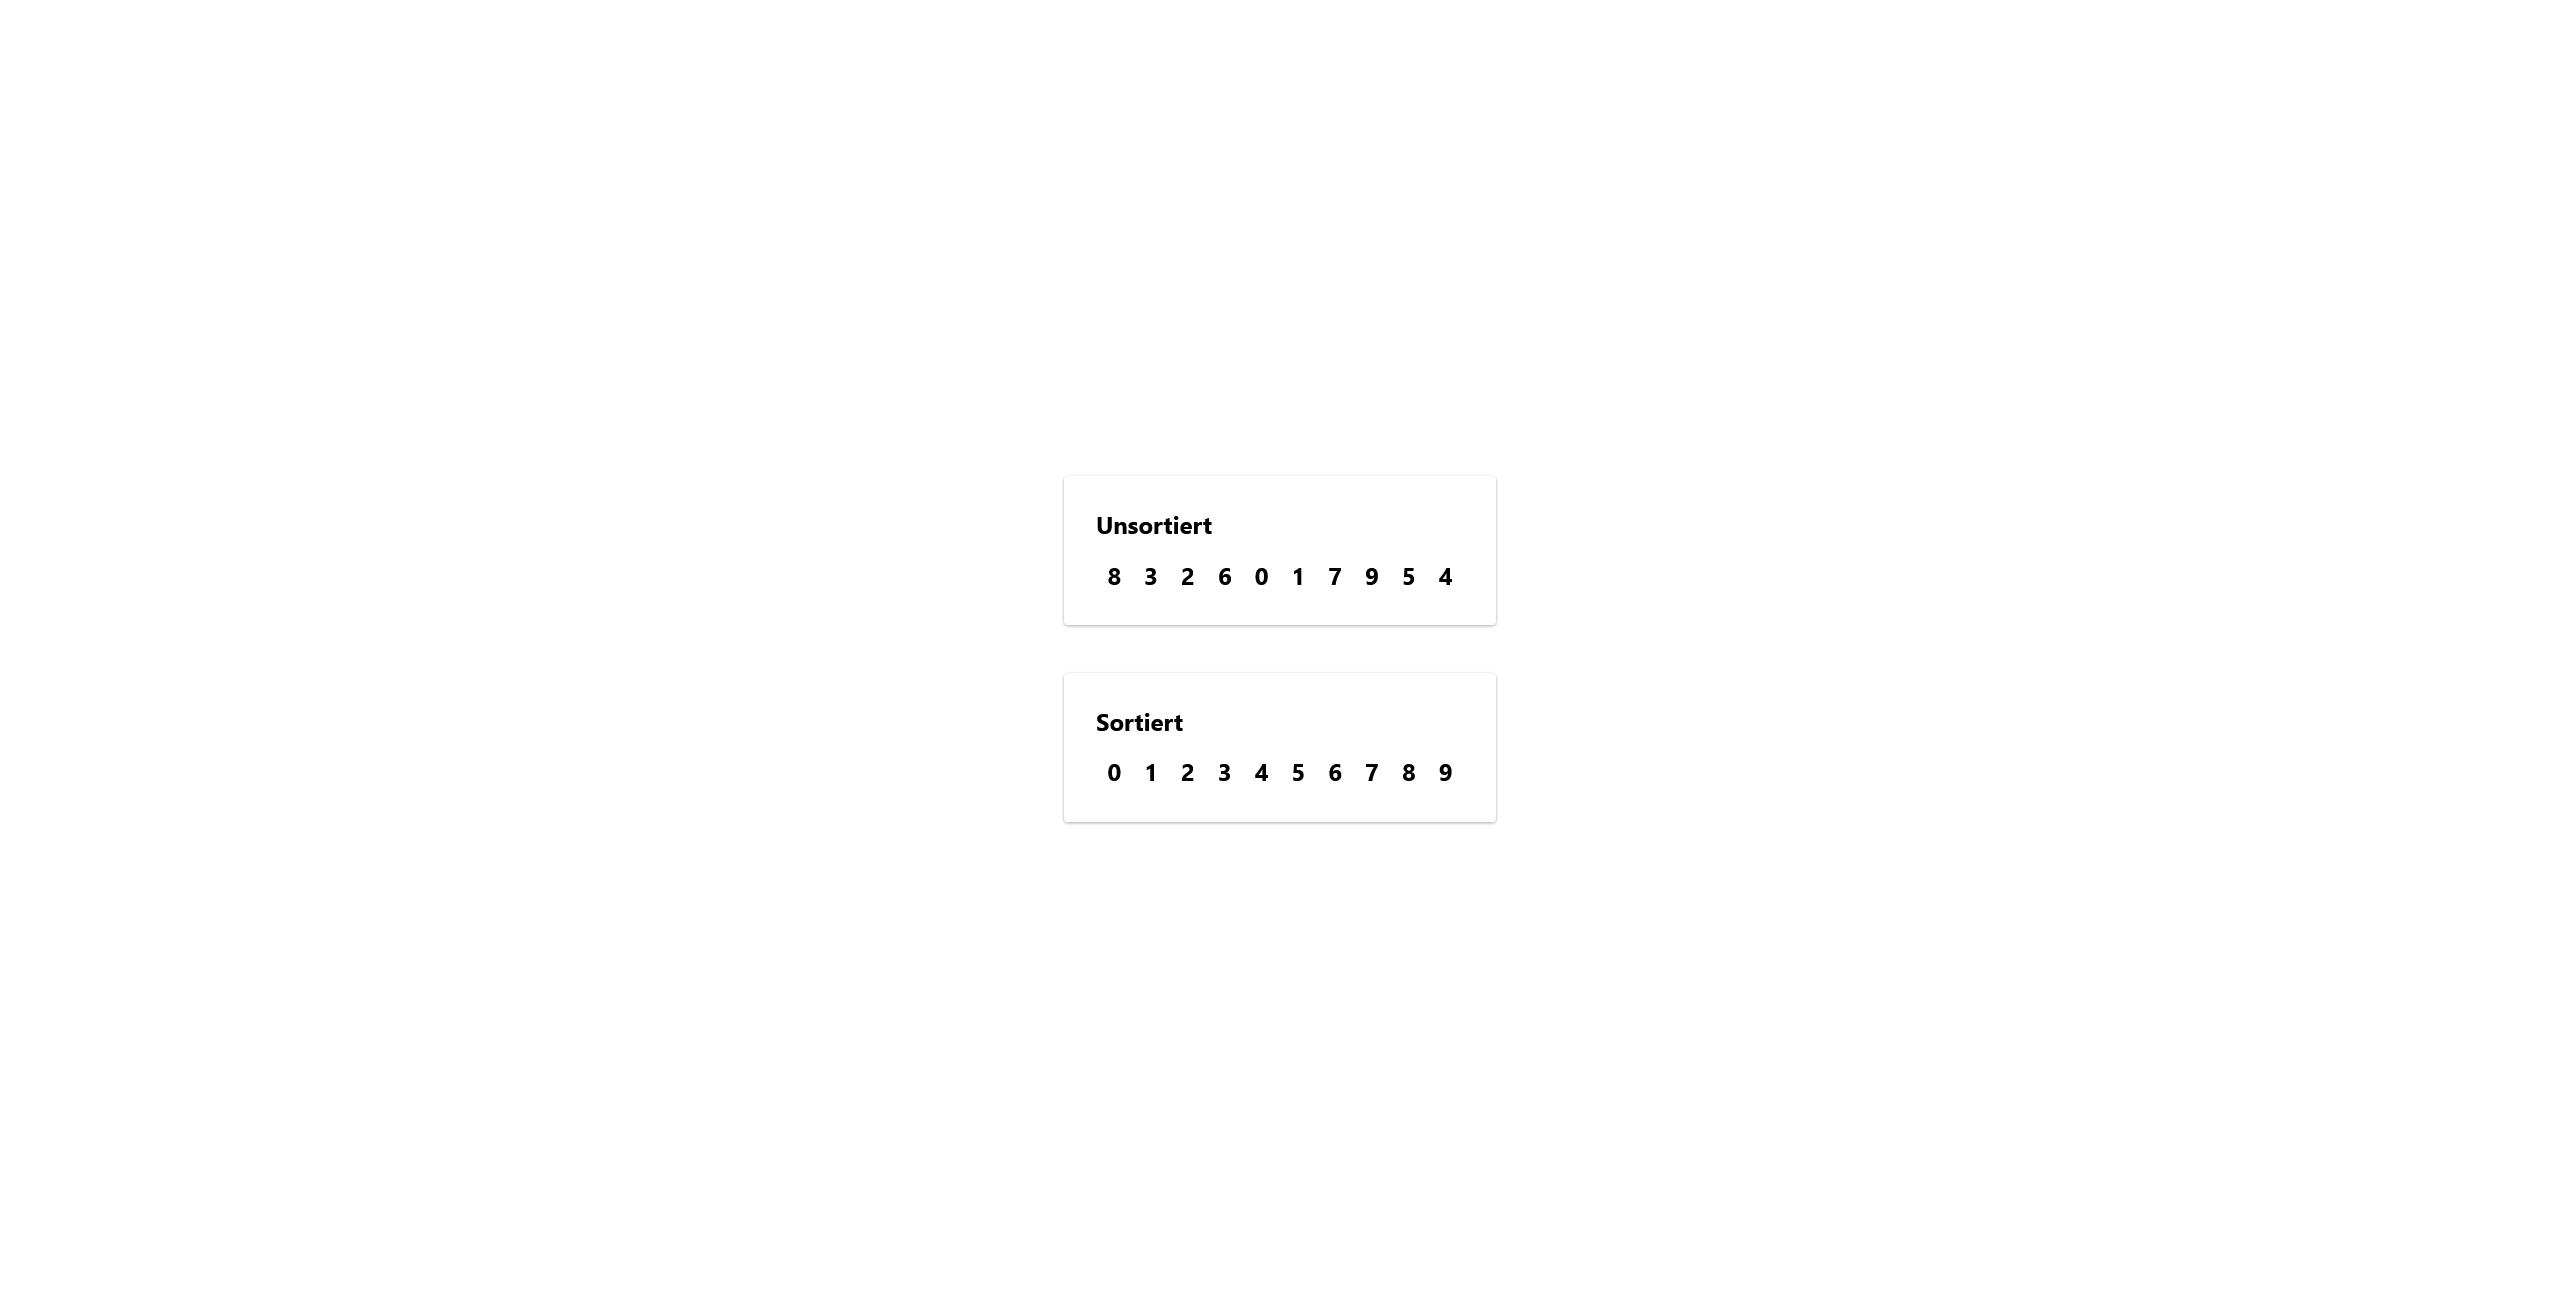
\includegraphics[width=\linewidth]{Abbildung-3}}
        \caption{Abbildung 3}
    \end{figure}

    \begin{figure}
        \centering
        \fbox{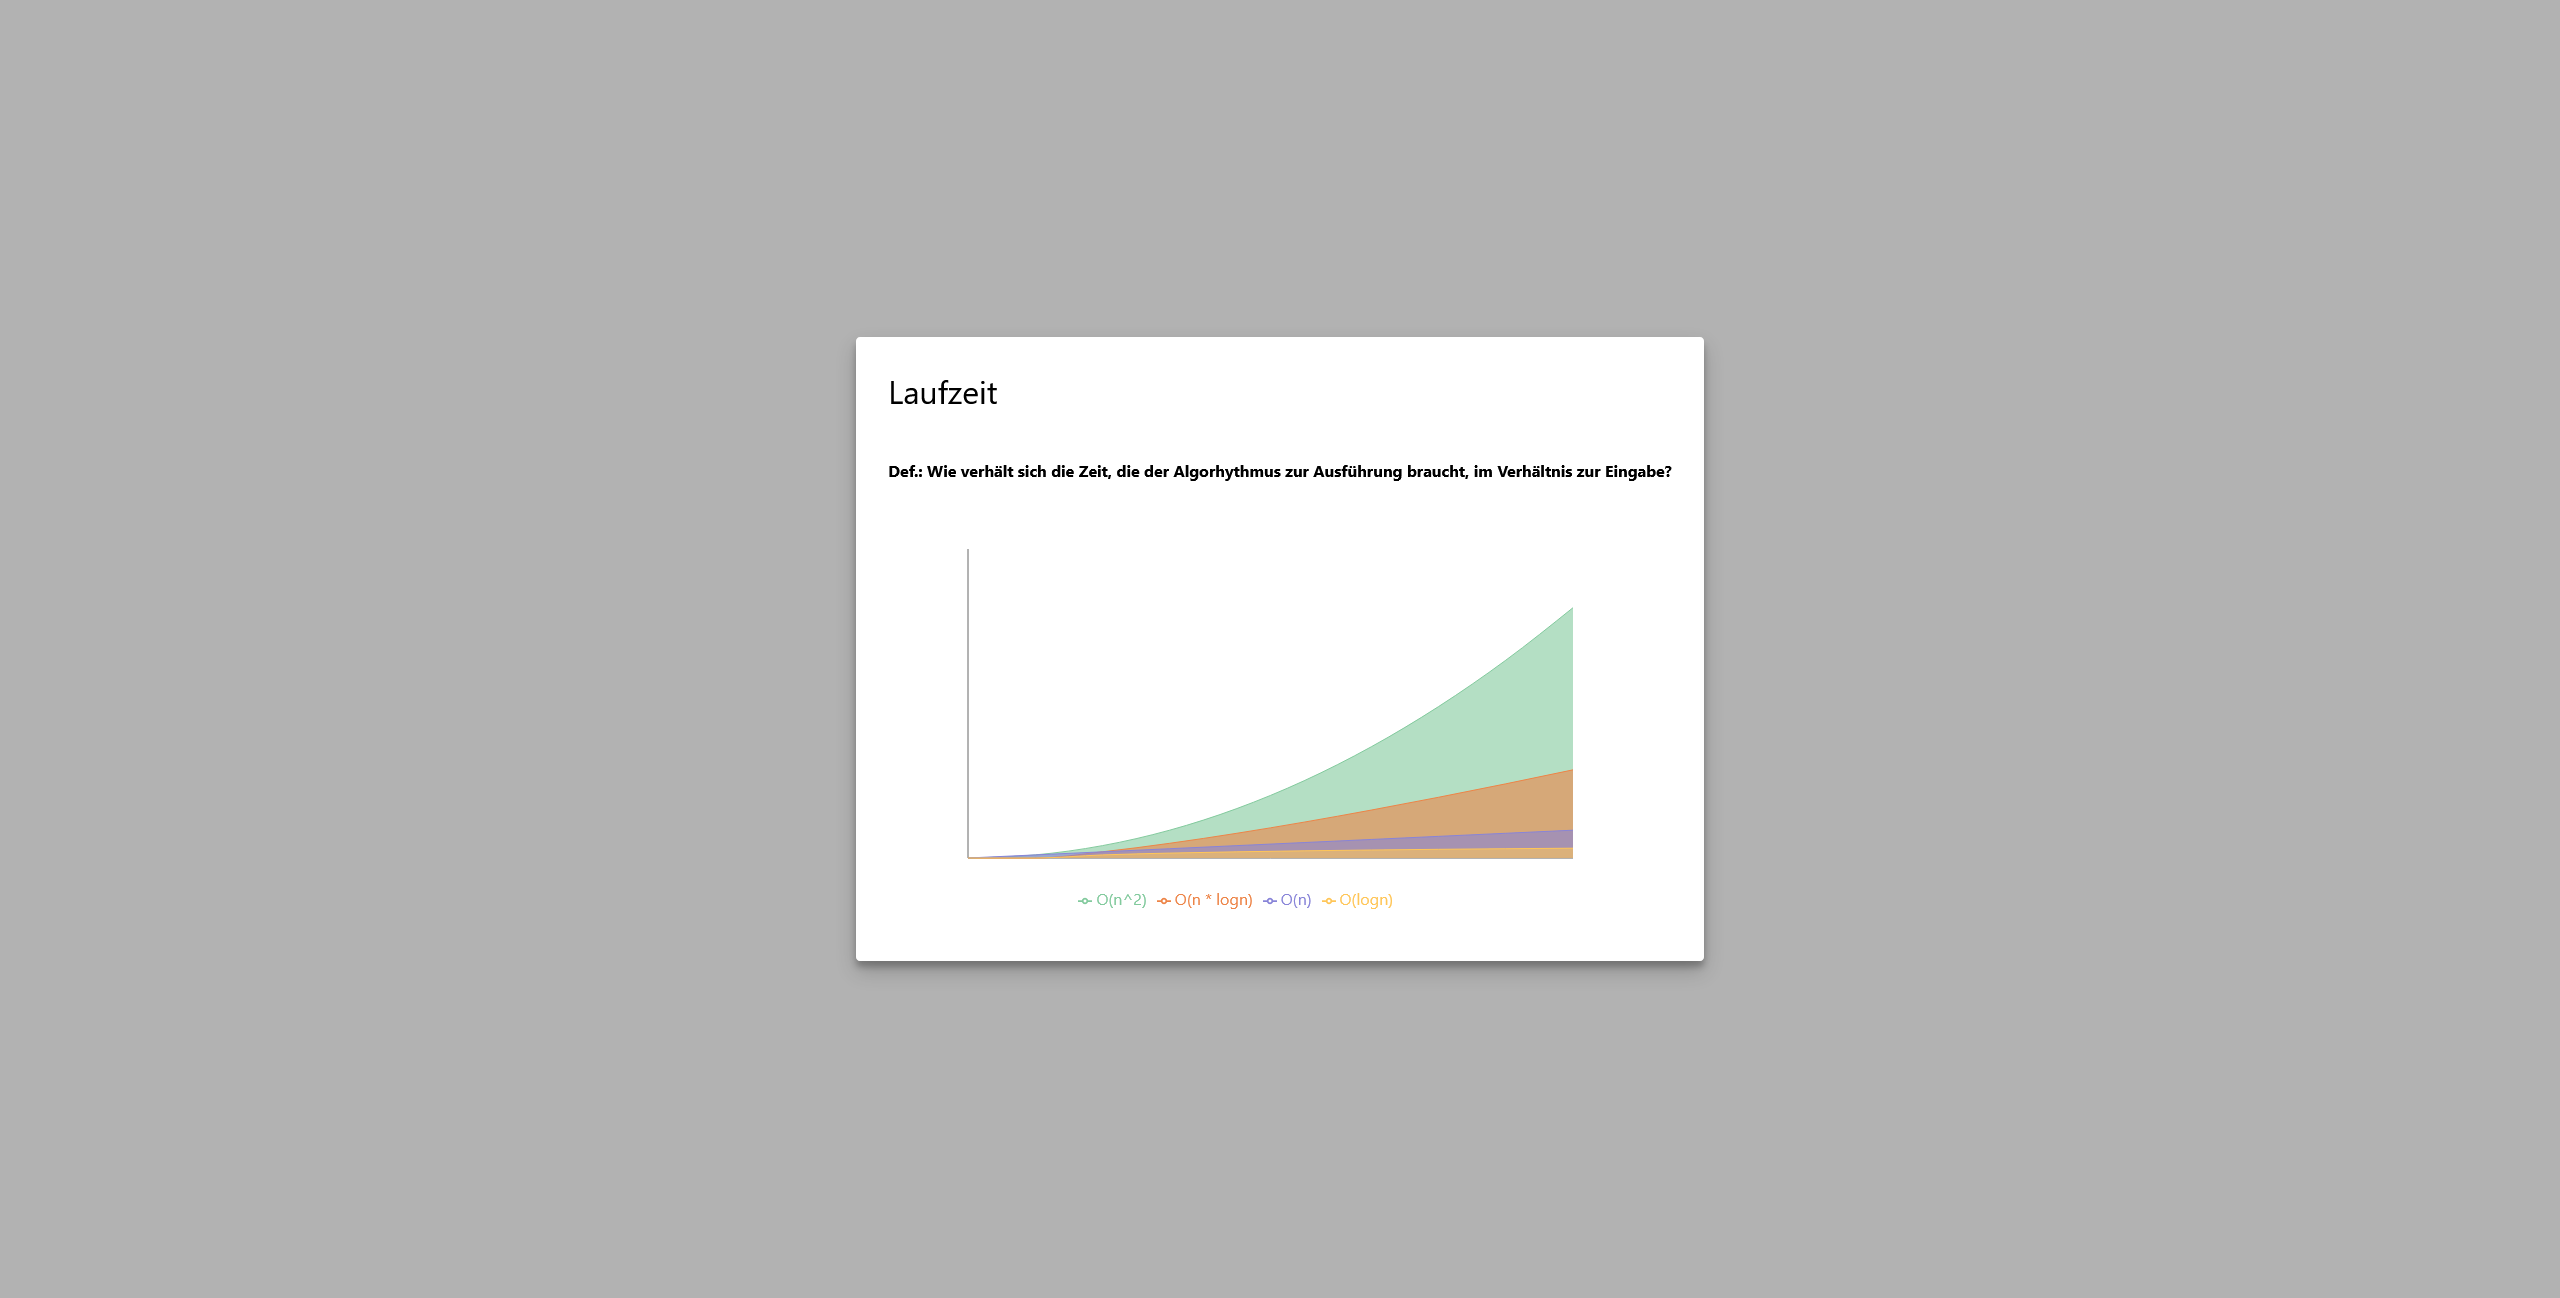
\includegraphics[width=\linewidth]{Abbildung-4}}
        \caption{Abbildung 4}
    \end{figure}

    \begin{figure}
        \centering
        \fbox{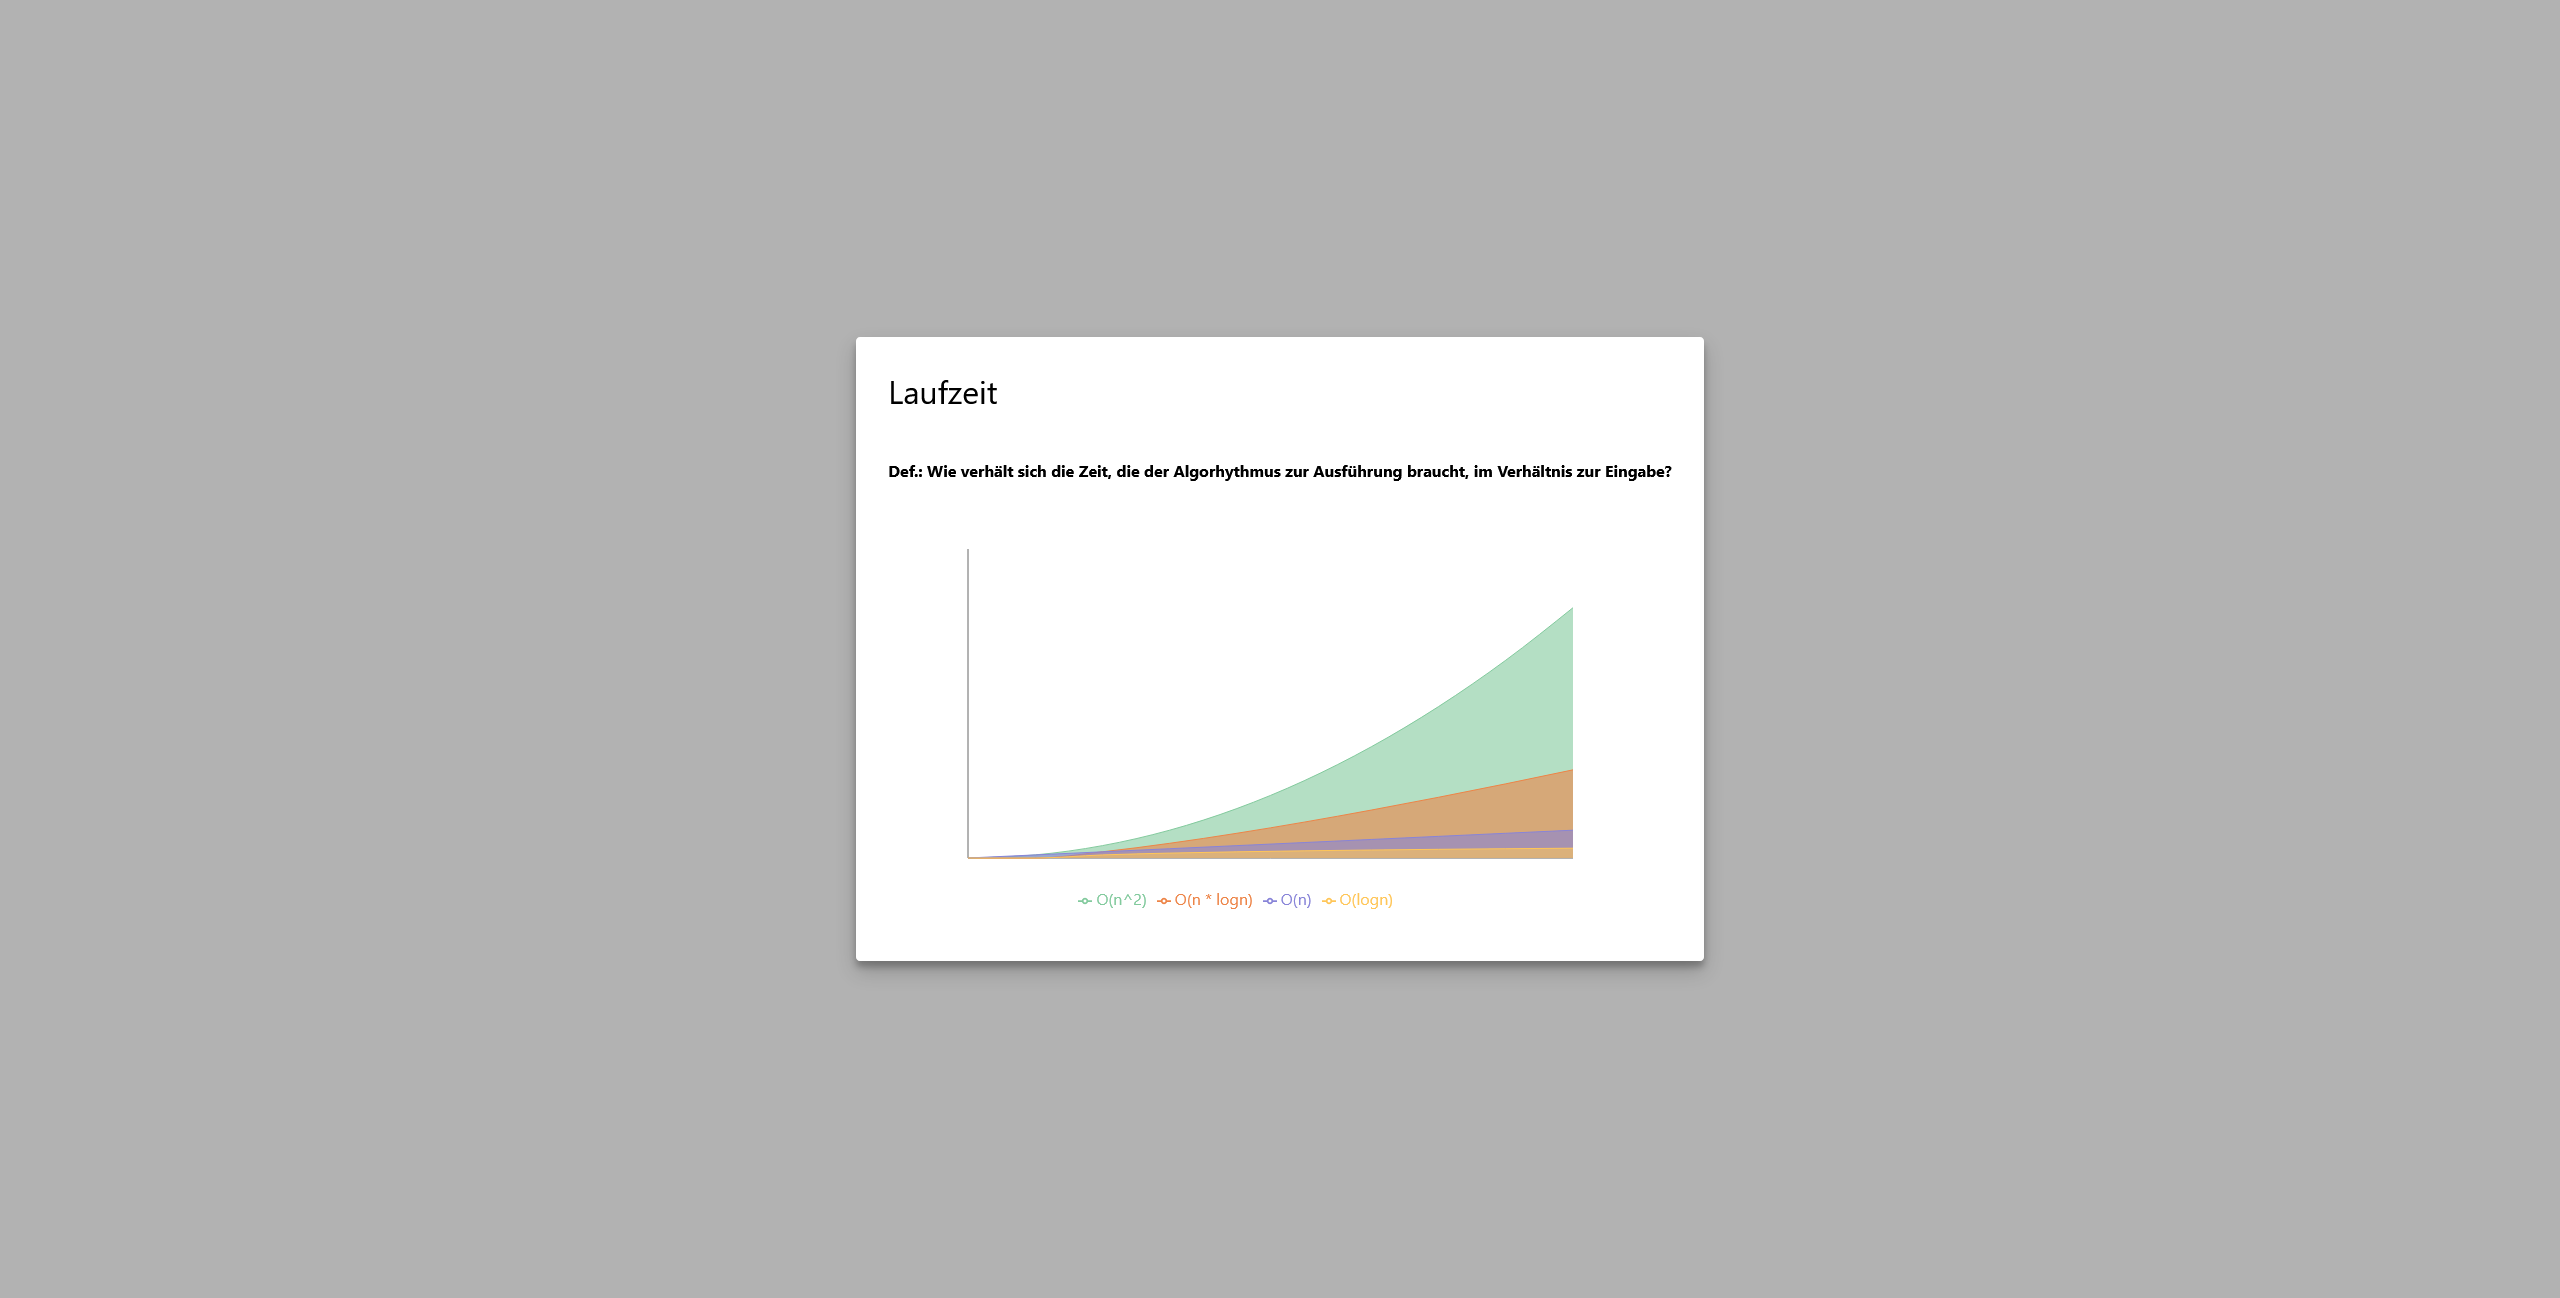
\includegraphics[width=\linewidth]{Abbildung-5}}
        \caption{Abbildung 5}
    \end{figure}

    \begin{figure}
        \centering
        \fbox{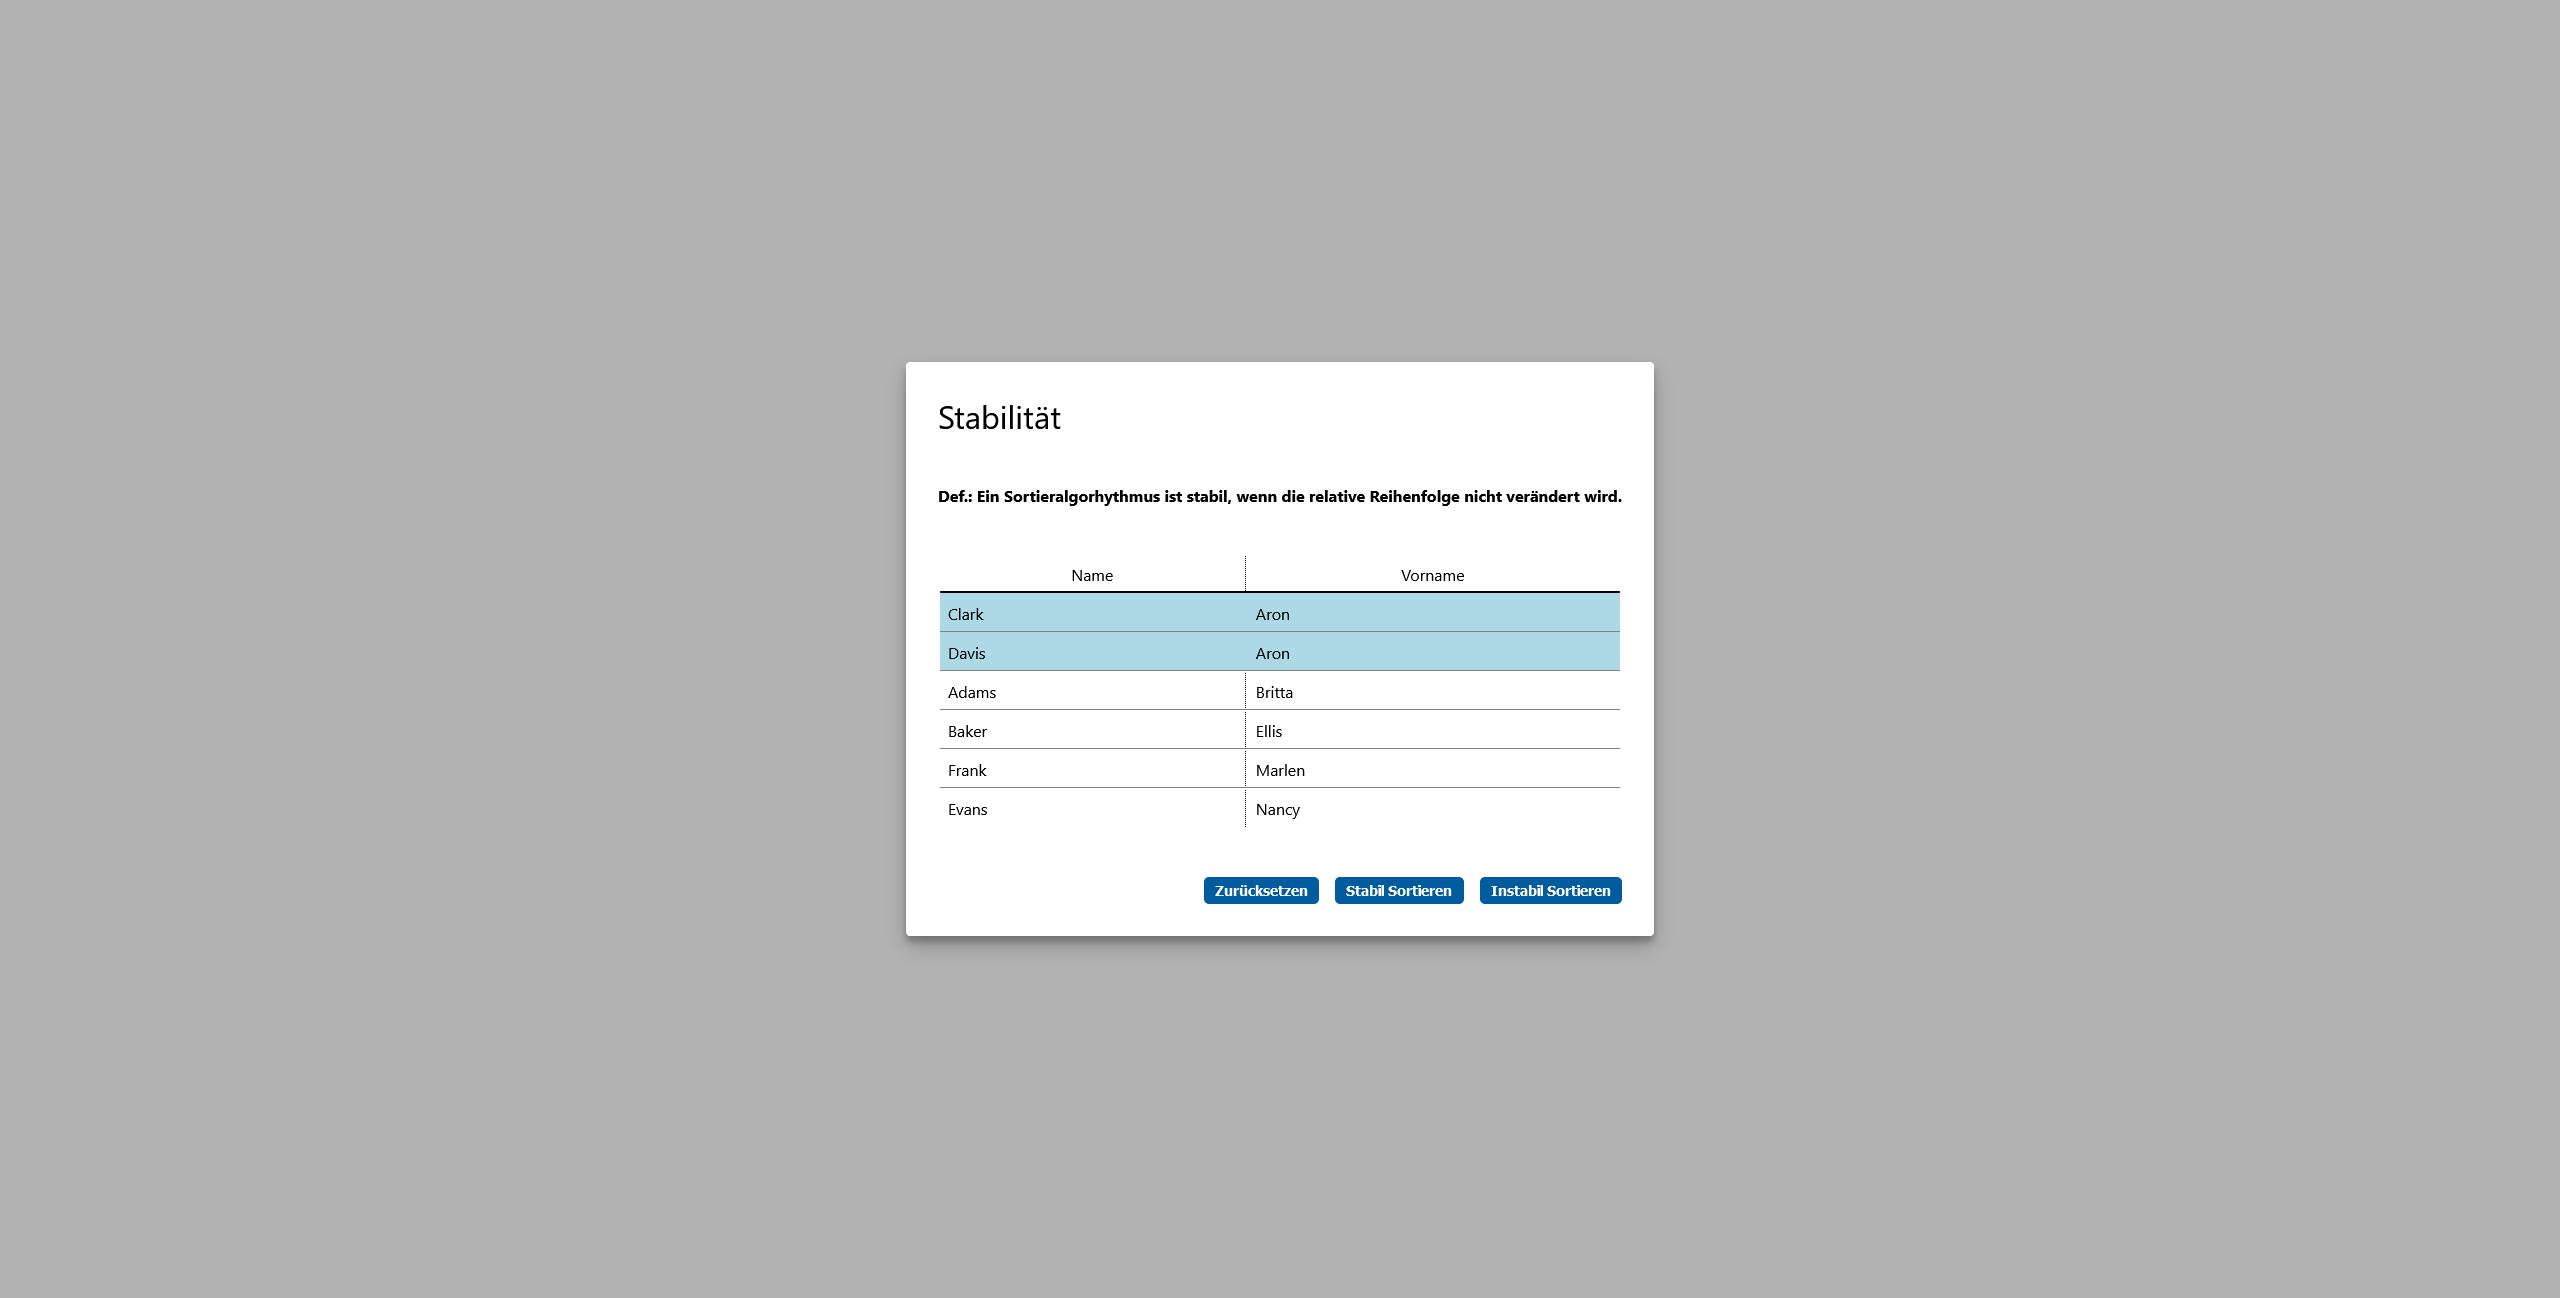
\includegraphics[width=\linewidth]{Abbildung-6}}
        \caption{Abbildung 6}
    \end{figure}

    \begin{figure}
        \centering
        \fbox{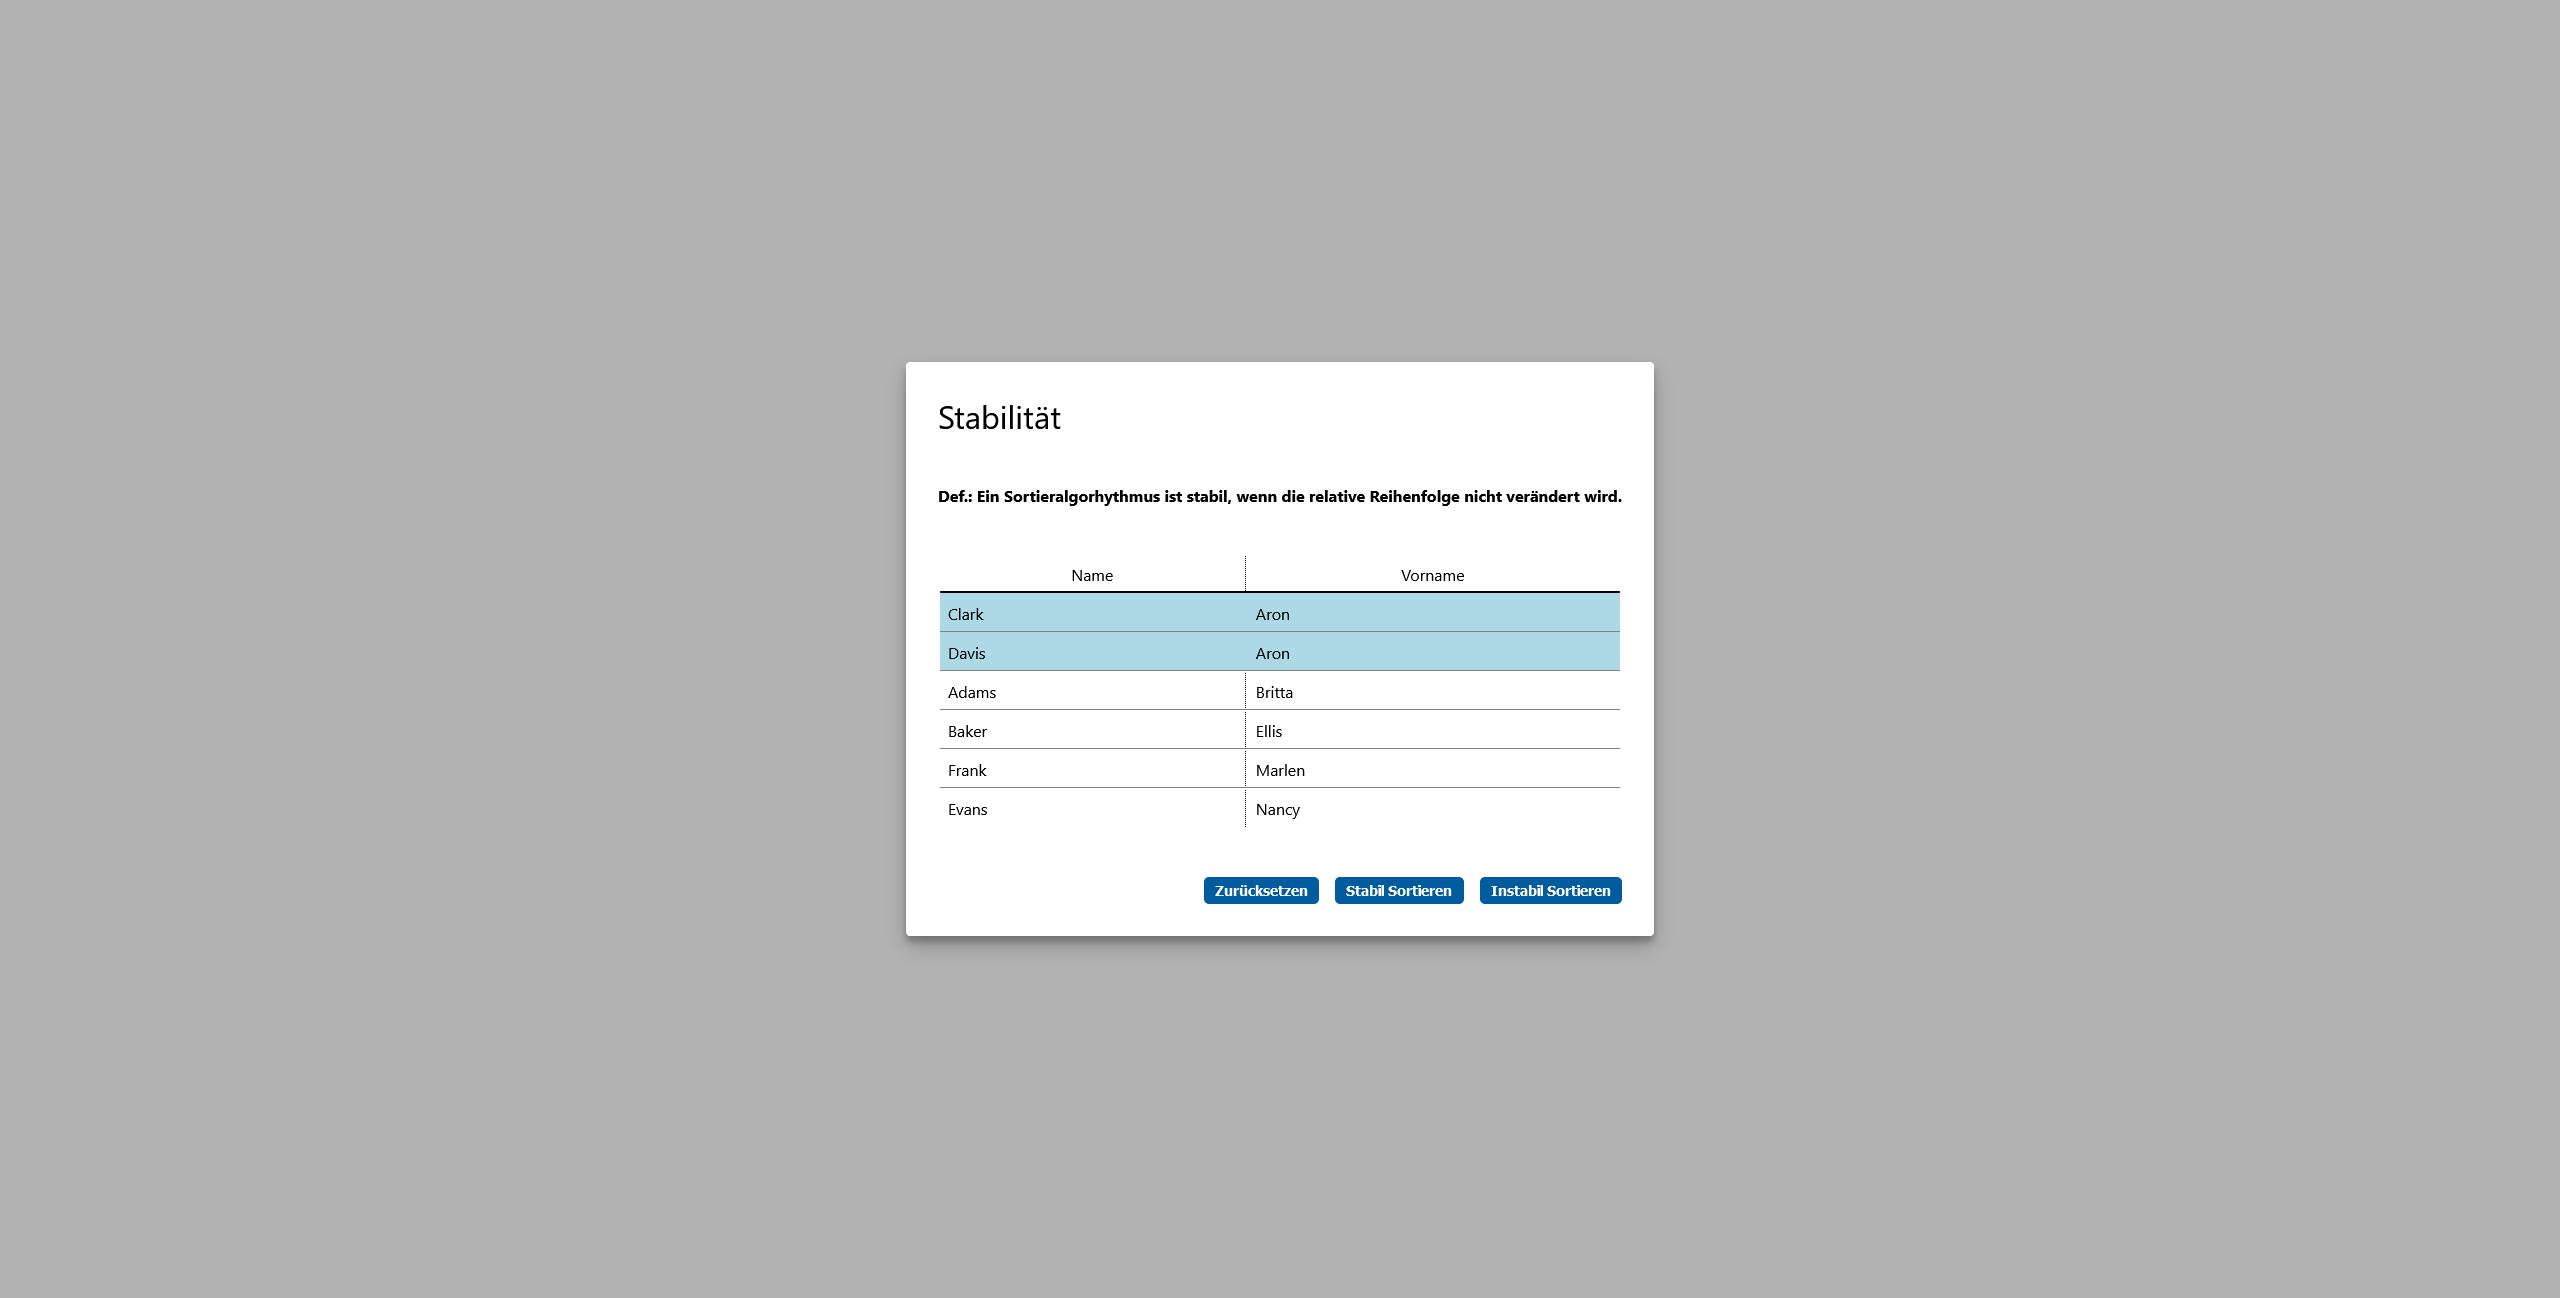
\includegraphics[width=\linewidth]{Abbildung-7}}
        \caption{Abbildung 7}
    \end{figure}

    \begin{figure}
        \centering
        \fbox{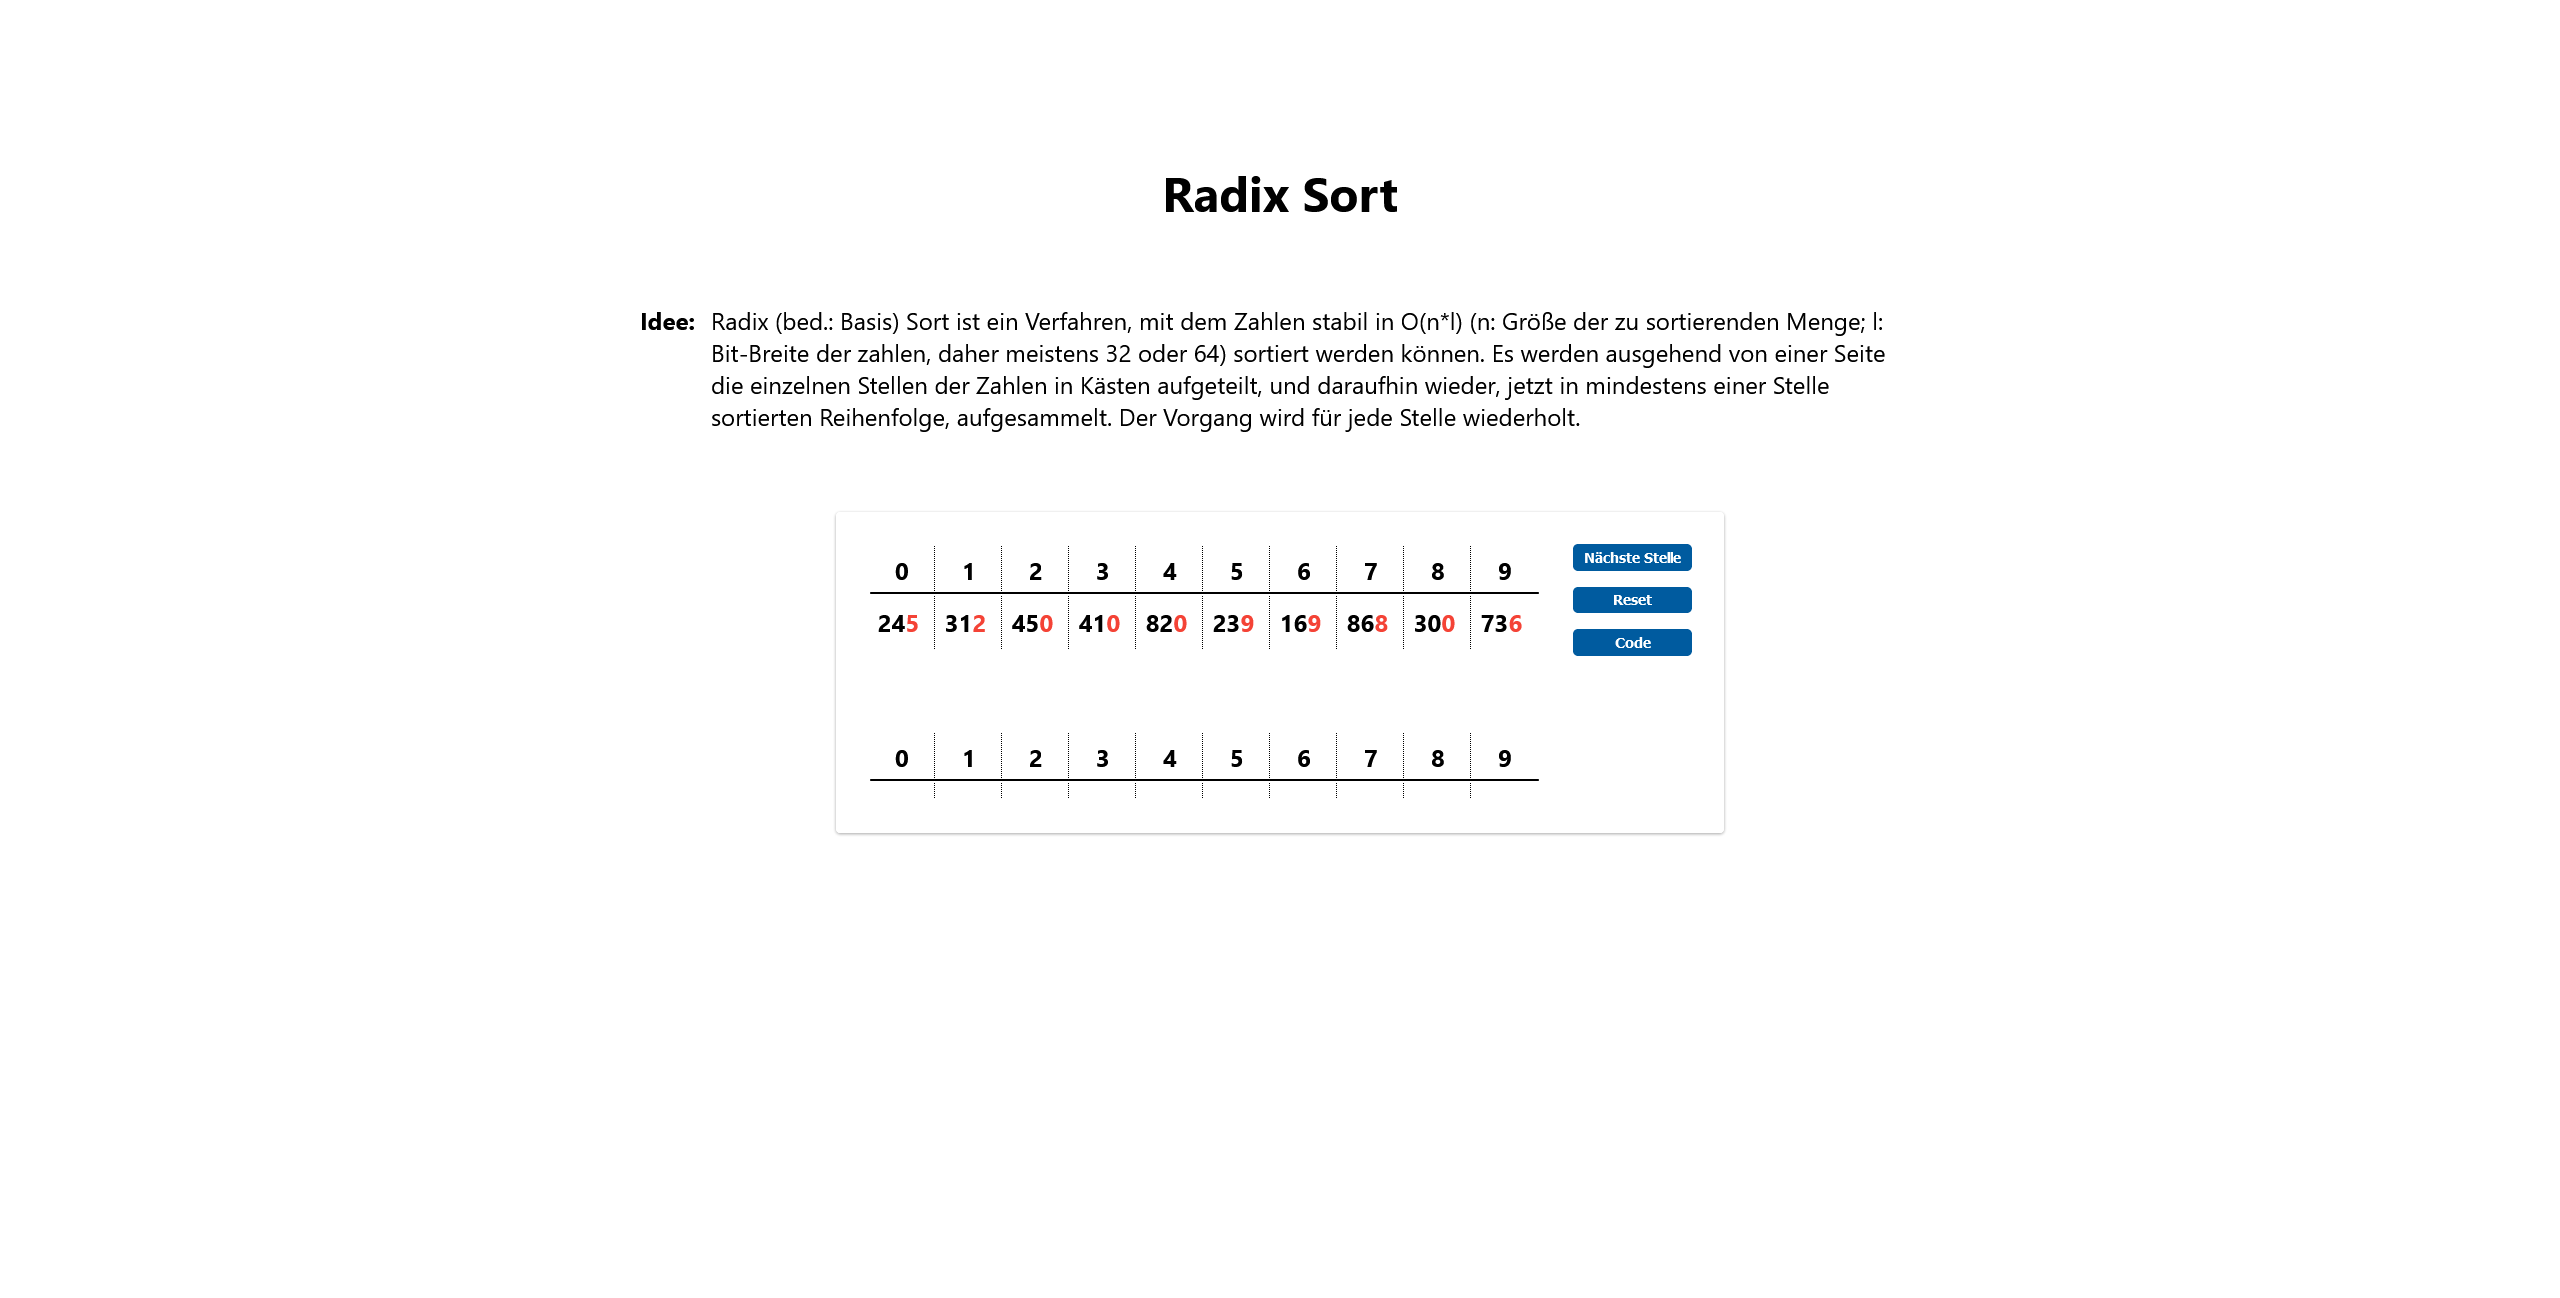
\includegraphics[width=\linewidth]{Abbildung-8}}
        \caption{Abbildung 8}
    \end{figure}

    \begin{figure}
        \centering
        \fbox{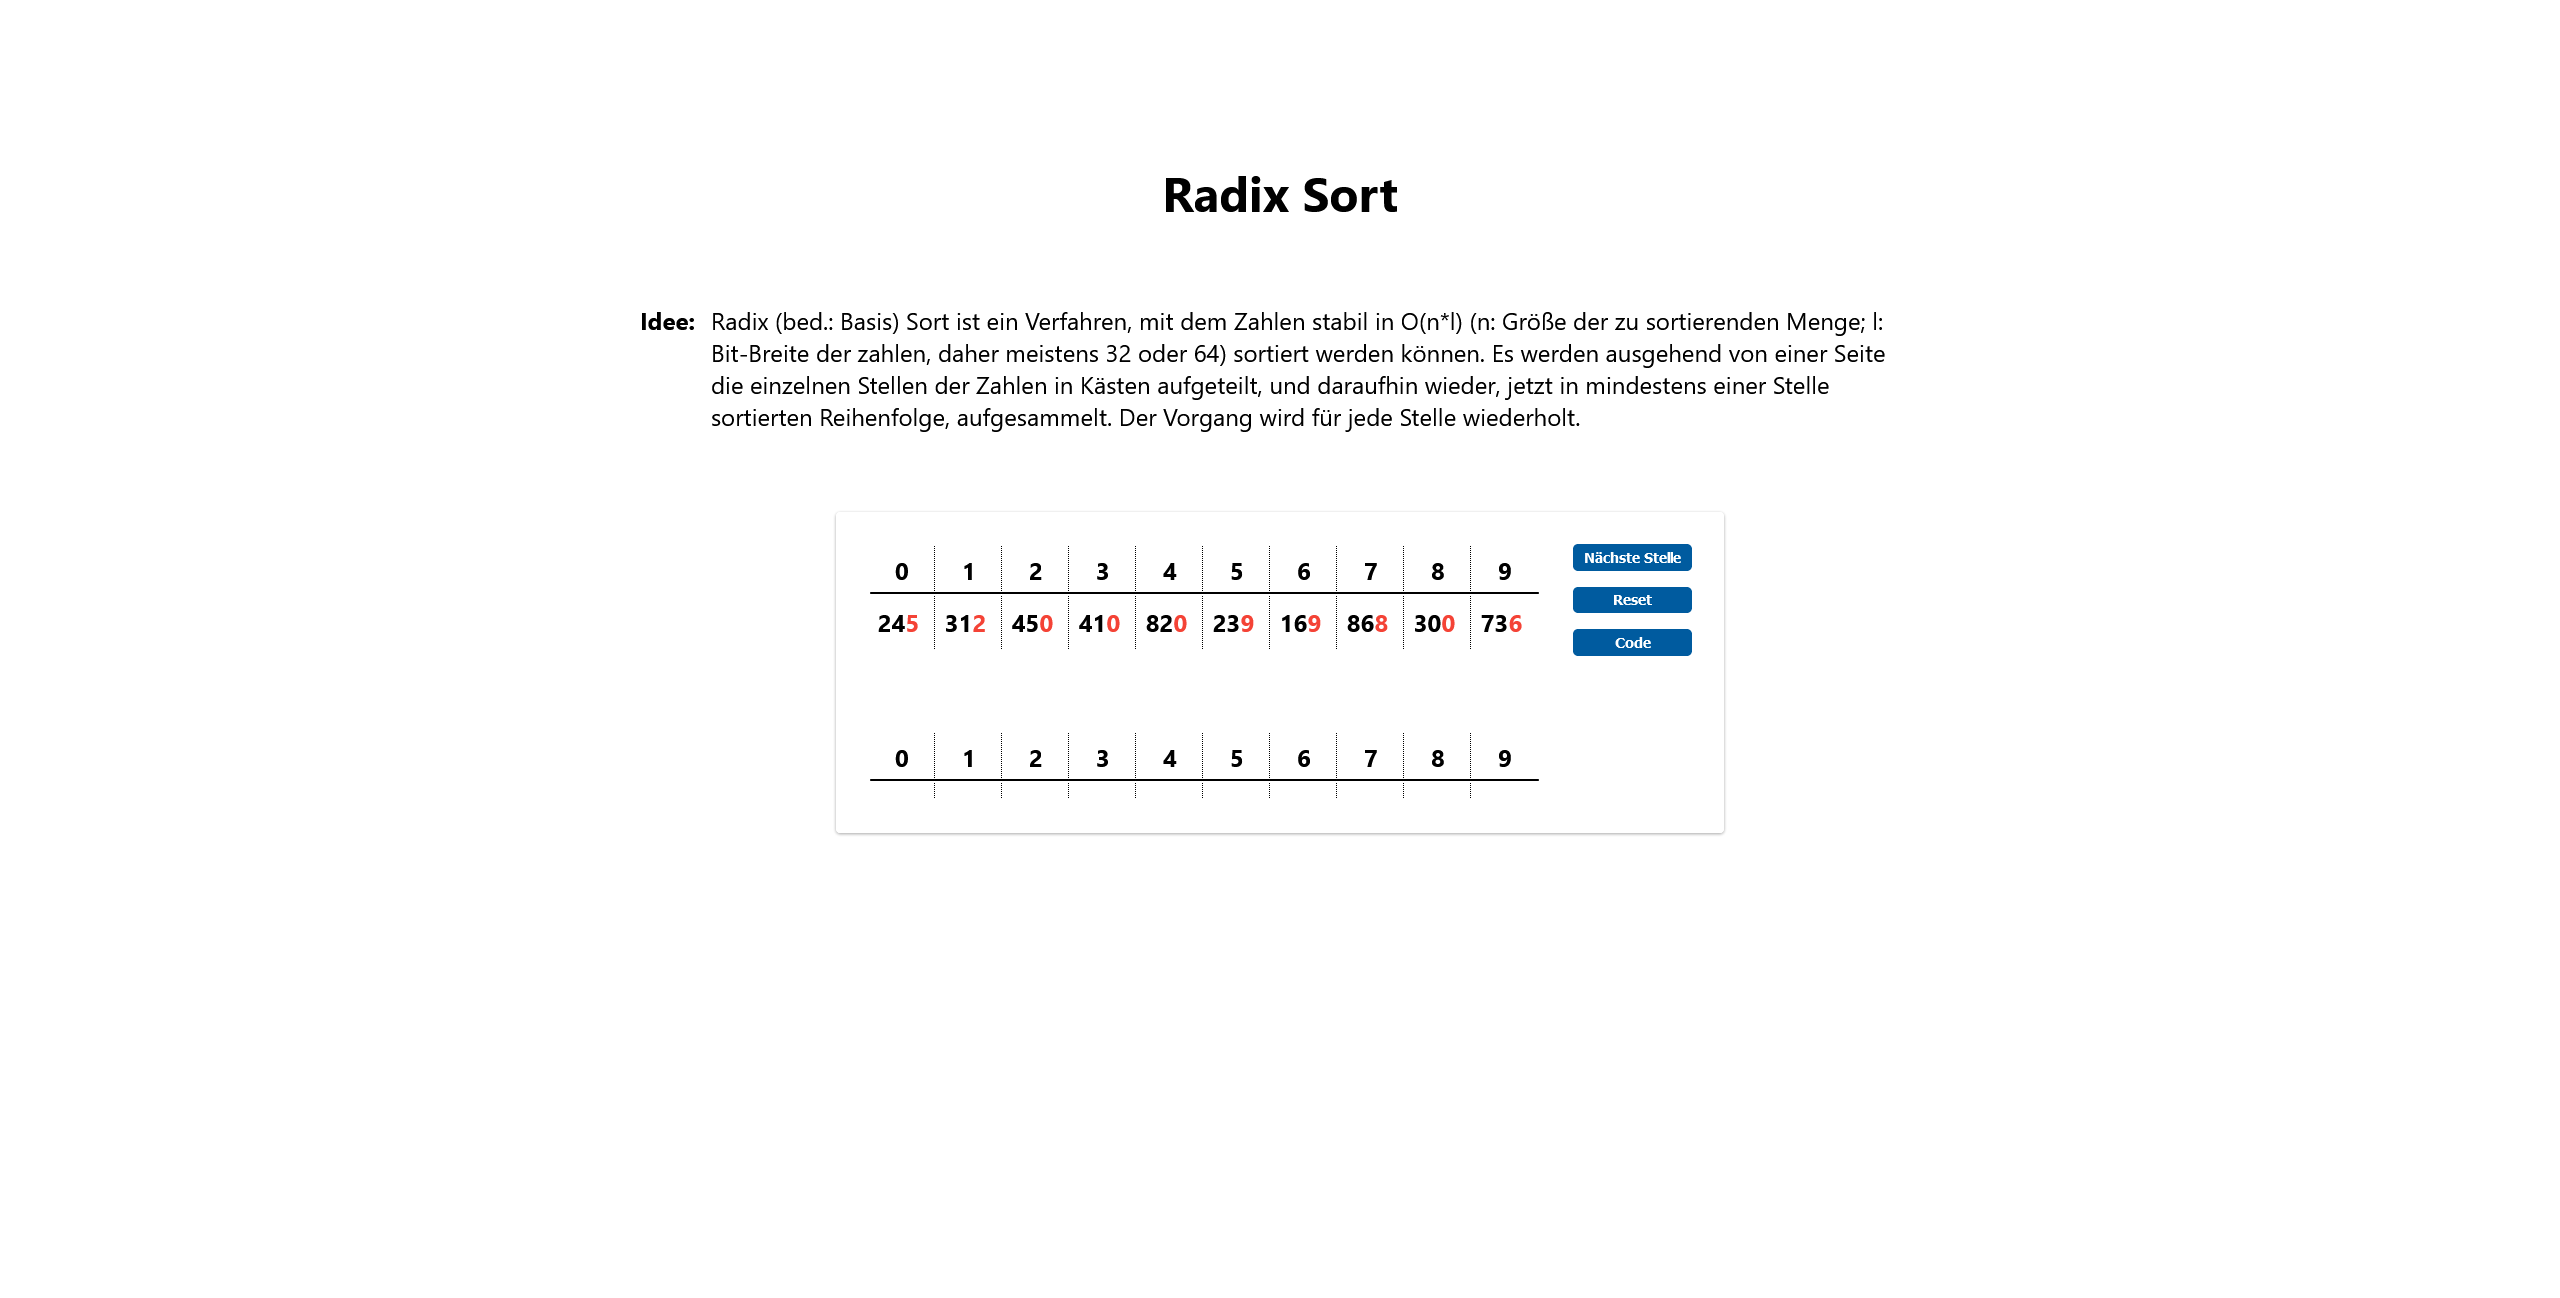
\includegraphics[width=\linewidth]{Abbildung-9}}
        \caption{Abbildung 9}
    \end{figure}

    \begin{figure}
        \centering
        \fbox{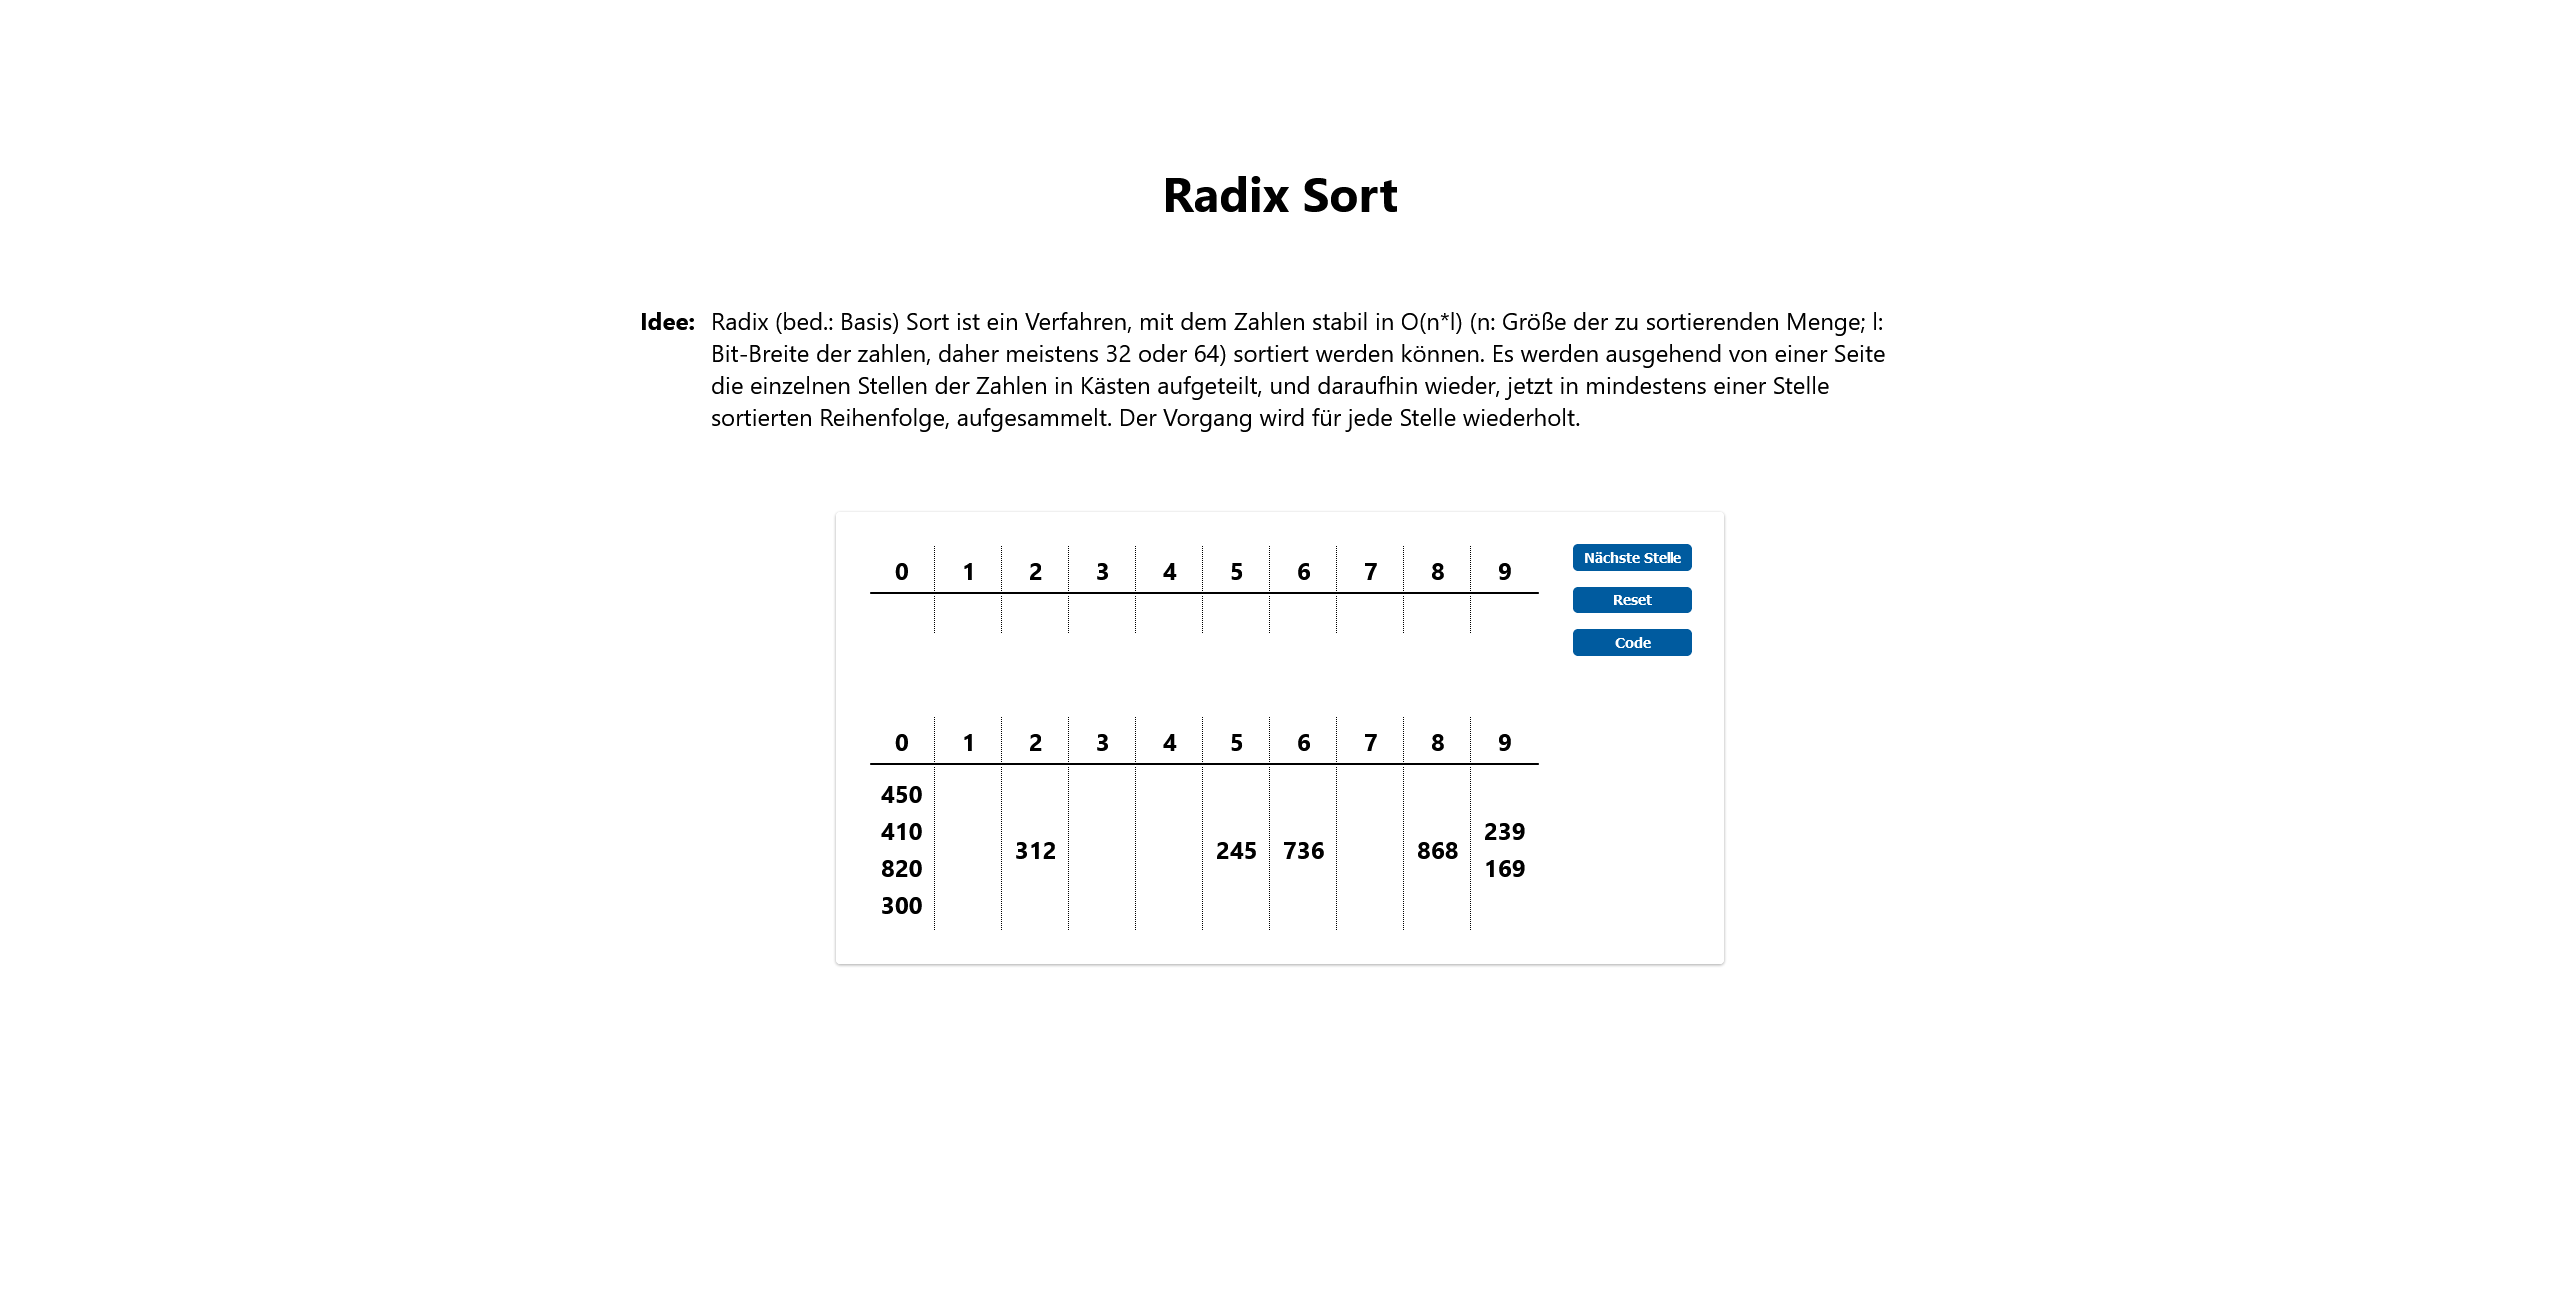
\includegraphics[width=\linewidth]{Abbildung-10}}
        \caption{Abbildung 10}
    \end{figure}

    \begin{figure}
        \centering
        \fbox{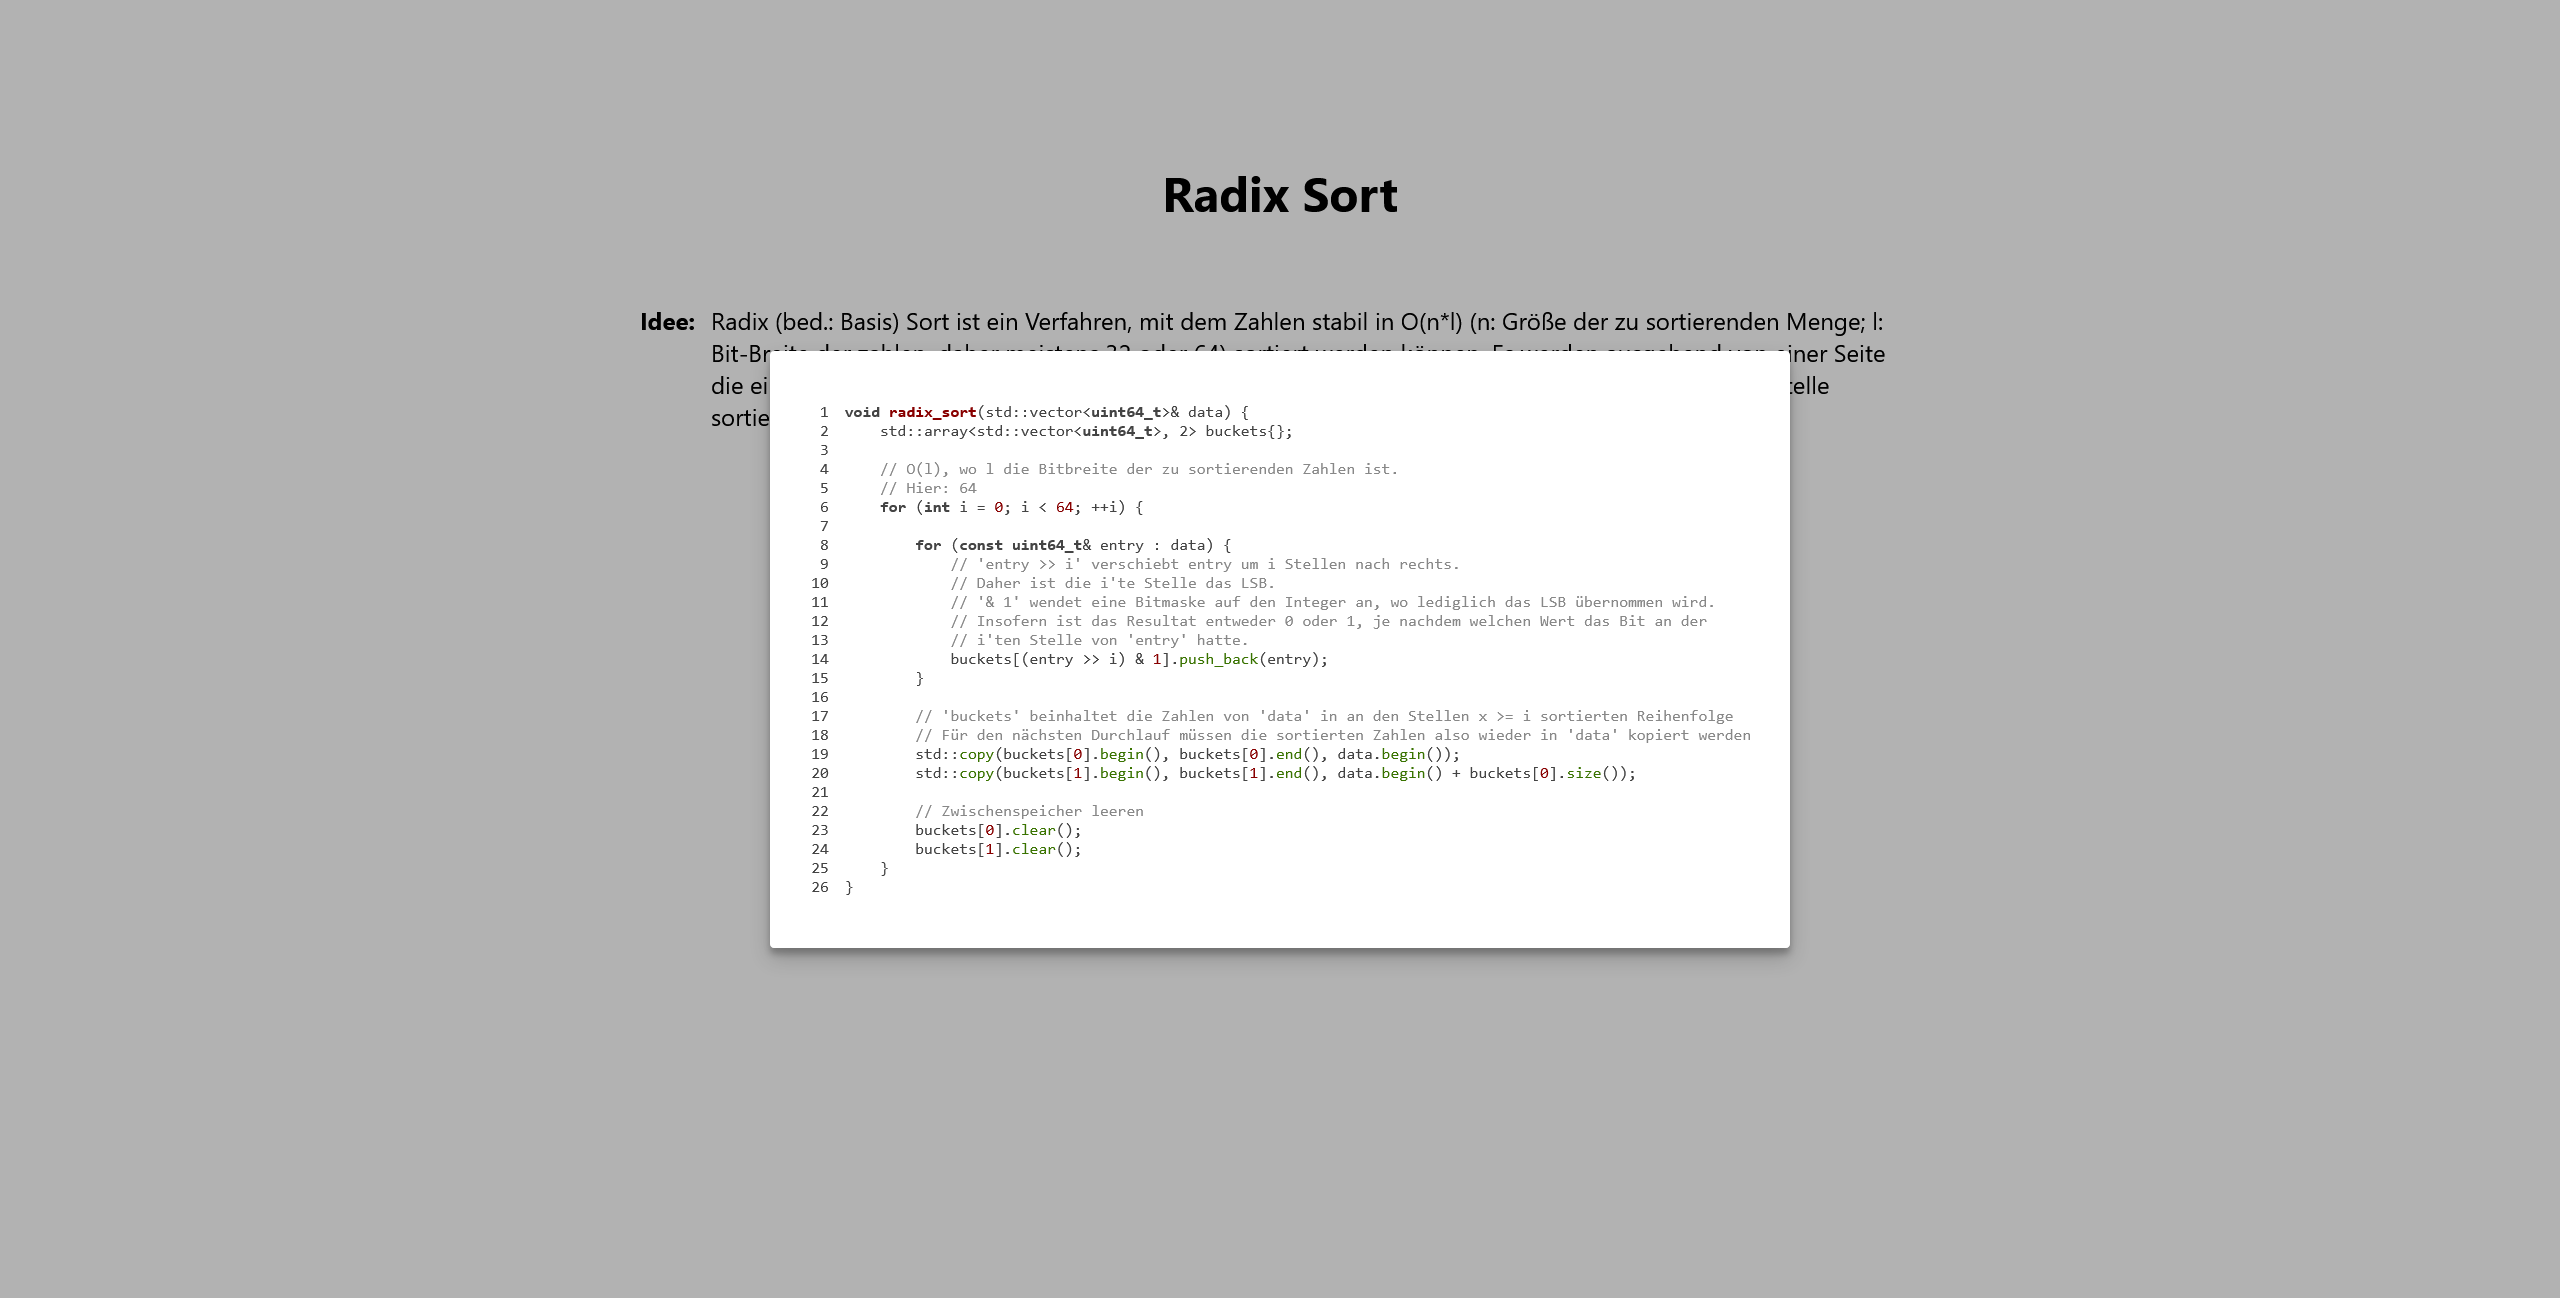
\includegraphics[width=\linewidth]{Abbildung-11}}
        \caption{Abbildung 11}
    \end{figure}

    \begin{figure}
        \centering
        \fbox{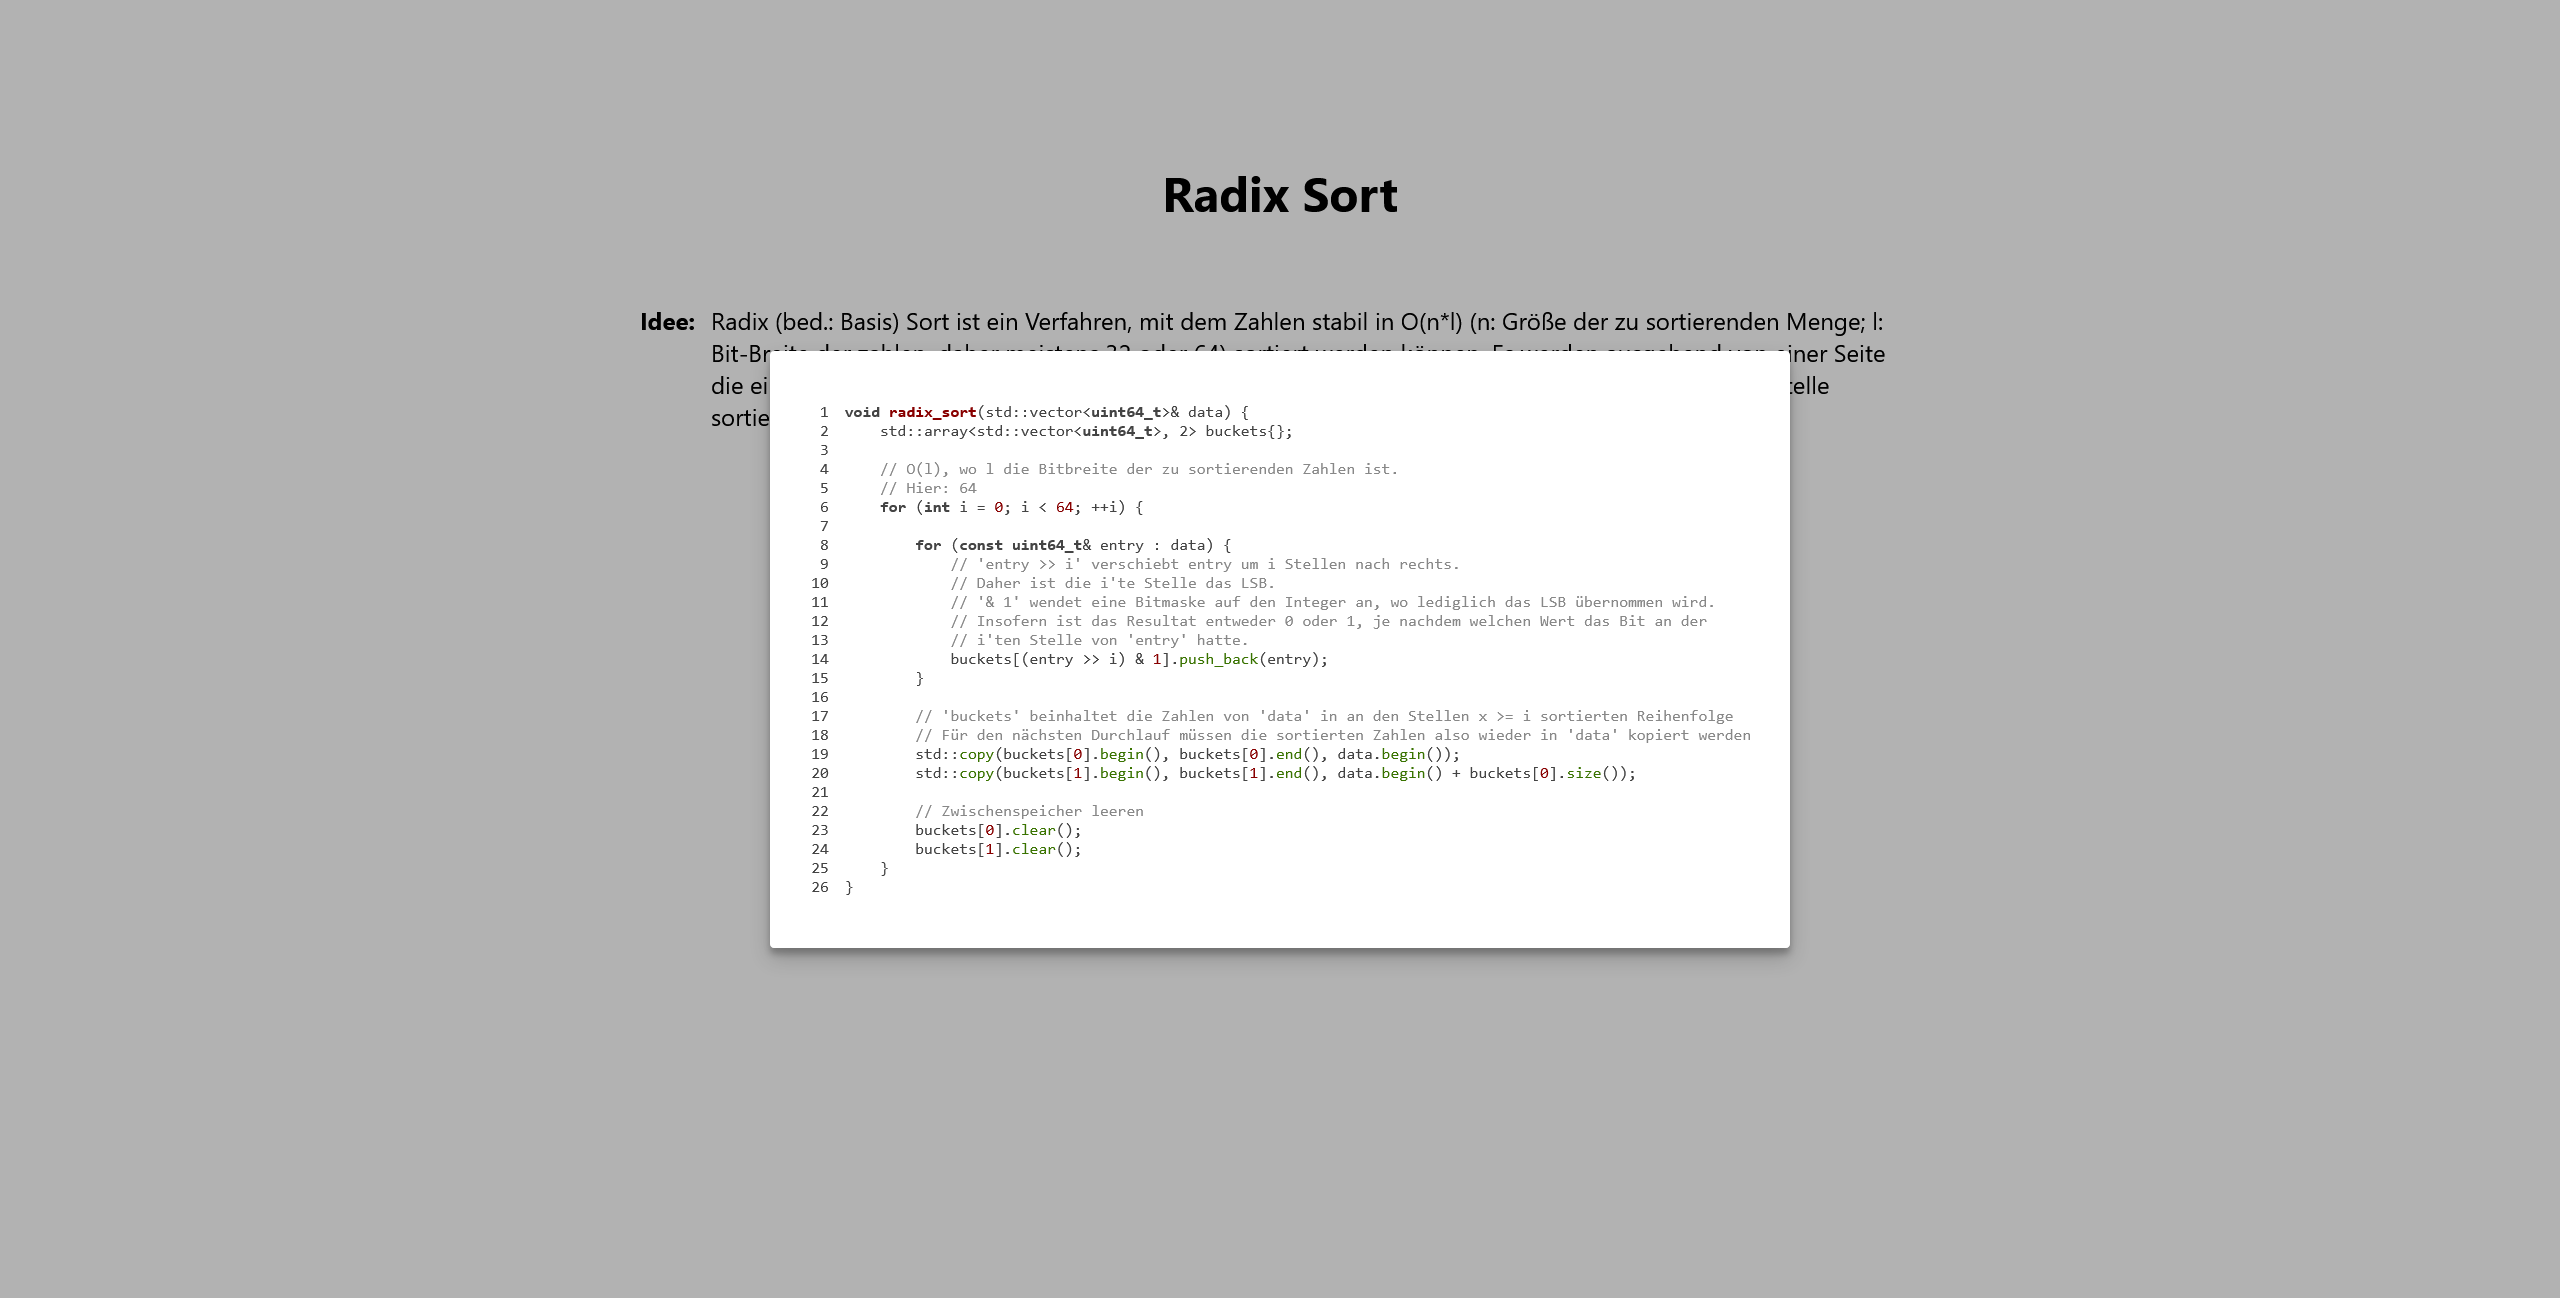
\includegraphics[width=\linewidth]{Abbildung-12}}
        \caption{Abbildung 12}
    \end{figure}

    \begin{figure}
        \centering
        \fbox{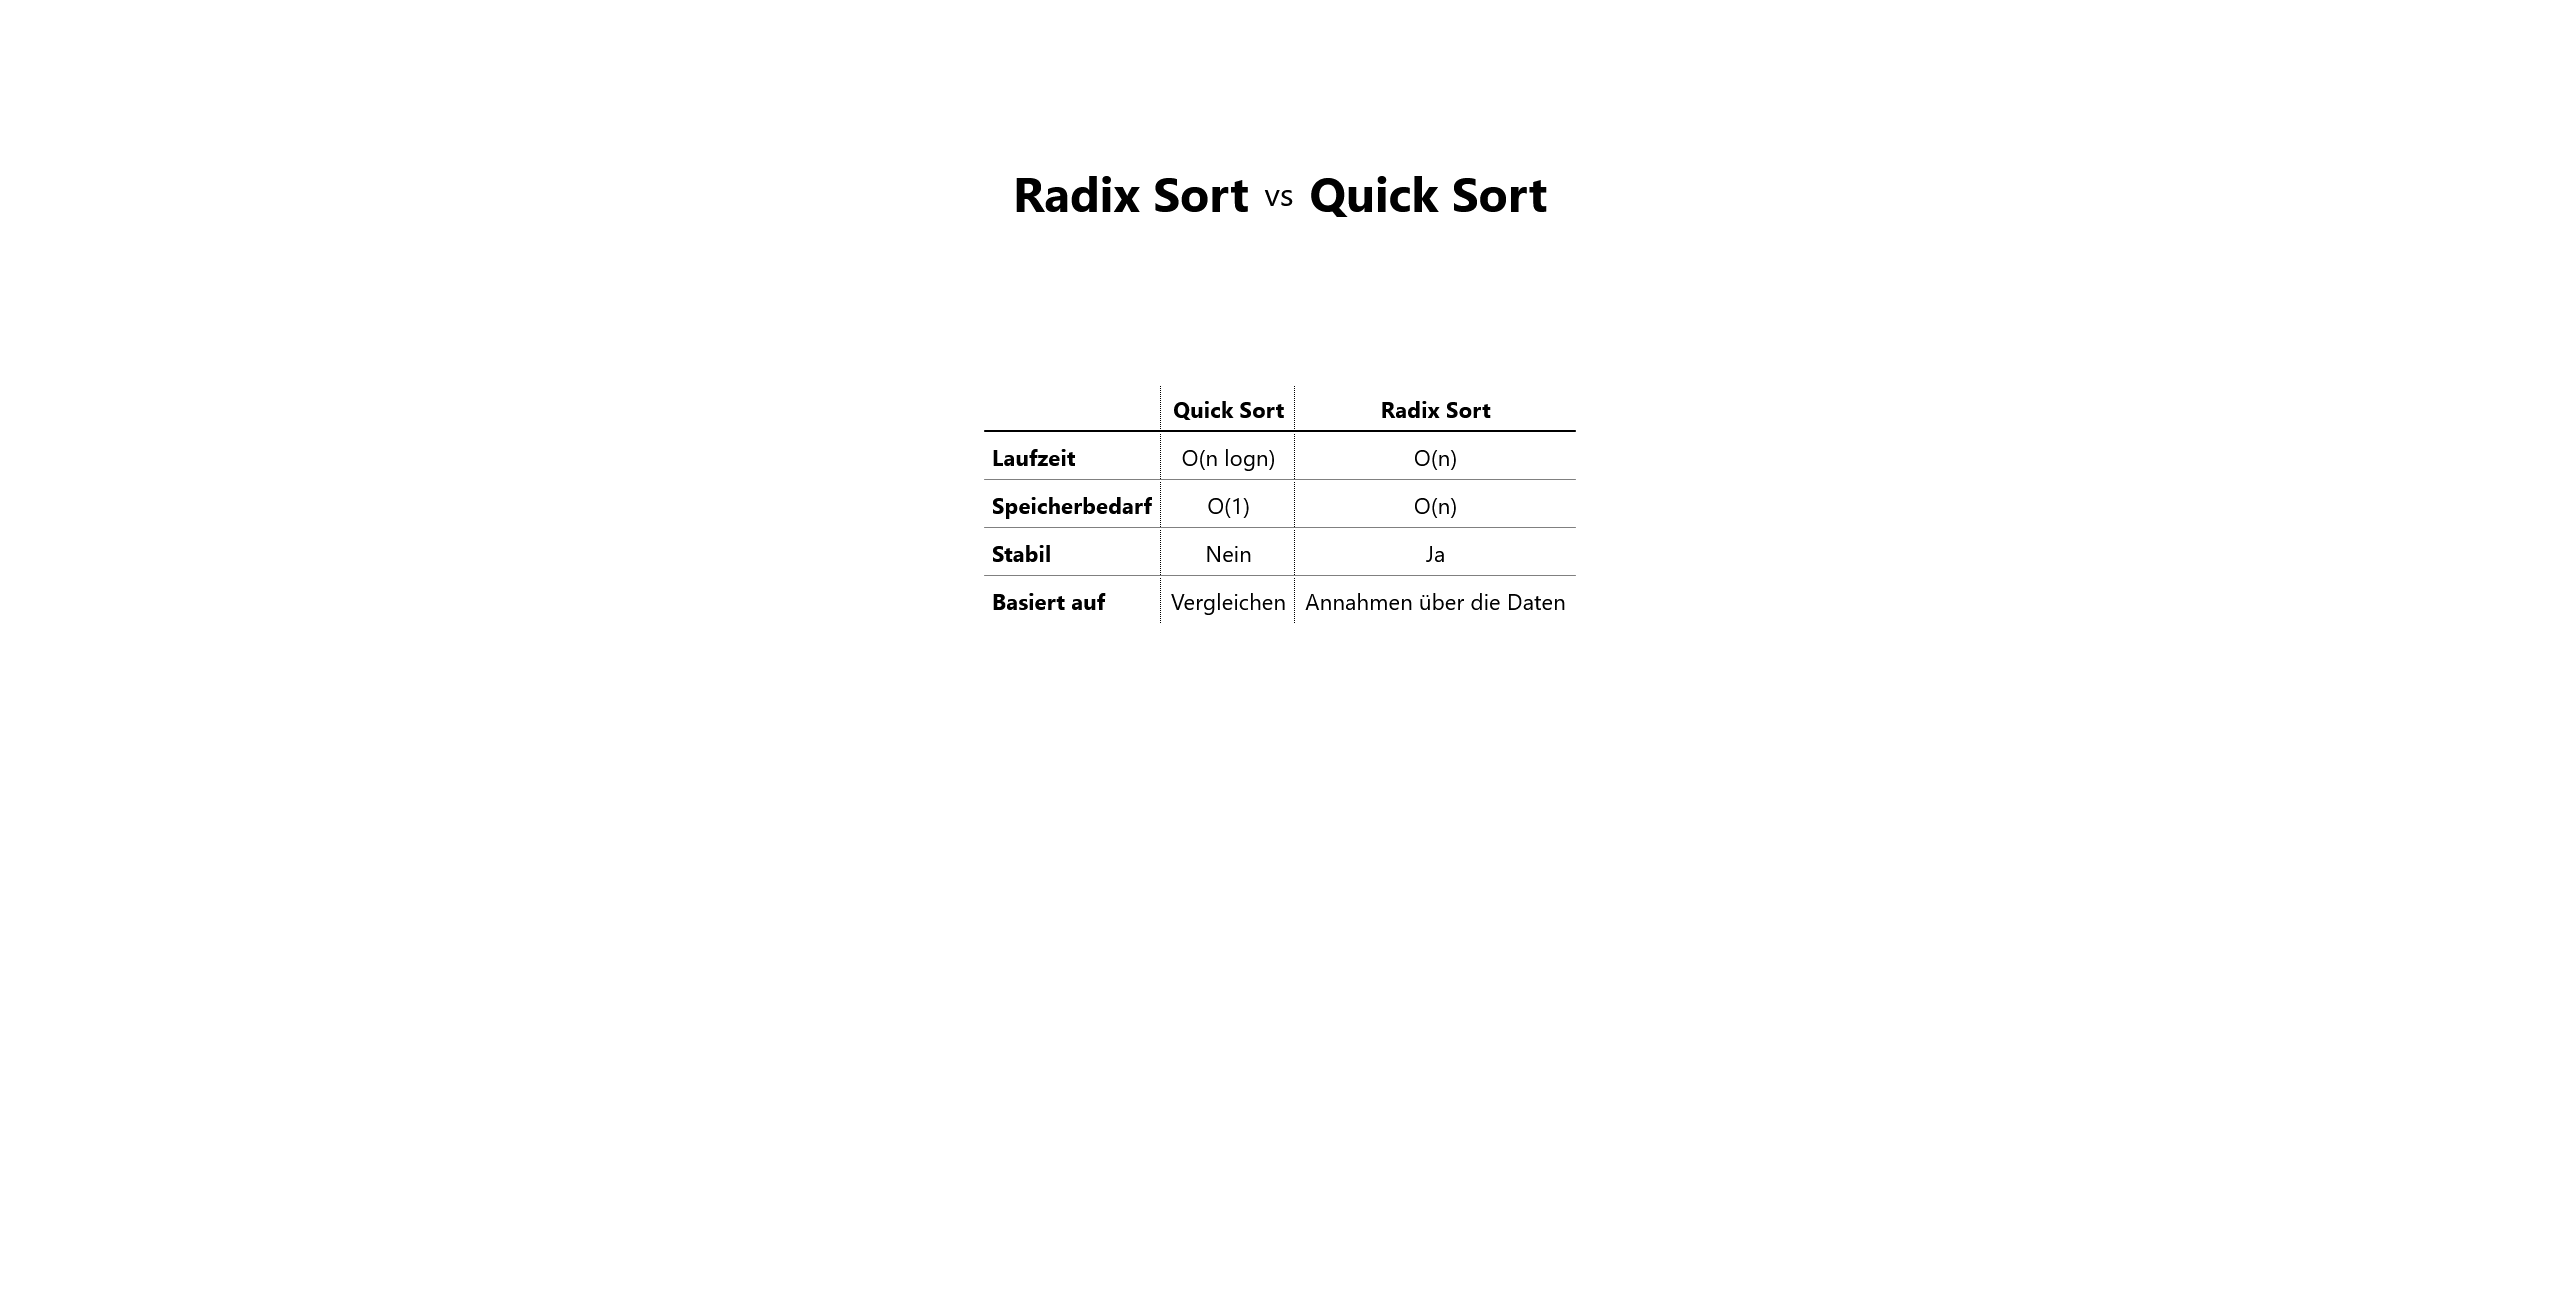
\includegraphics[width=\linewidth]{Abbildung-13}}
        \caption{Abbildung 13}
    \end{figure}

    \begin{figure}
        \centering
        \fbox{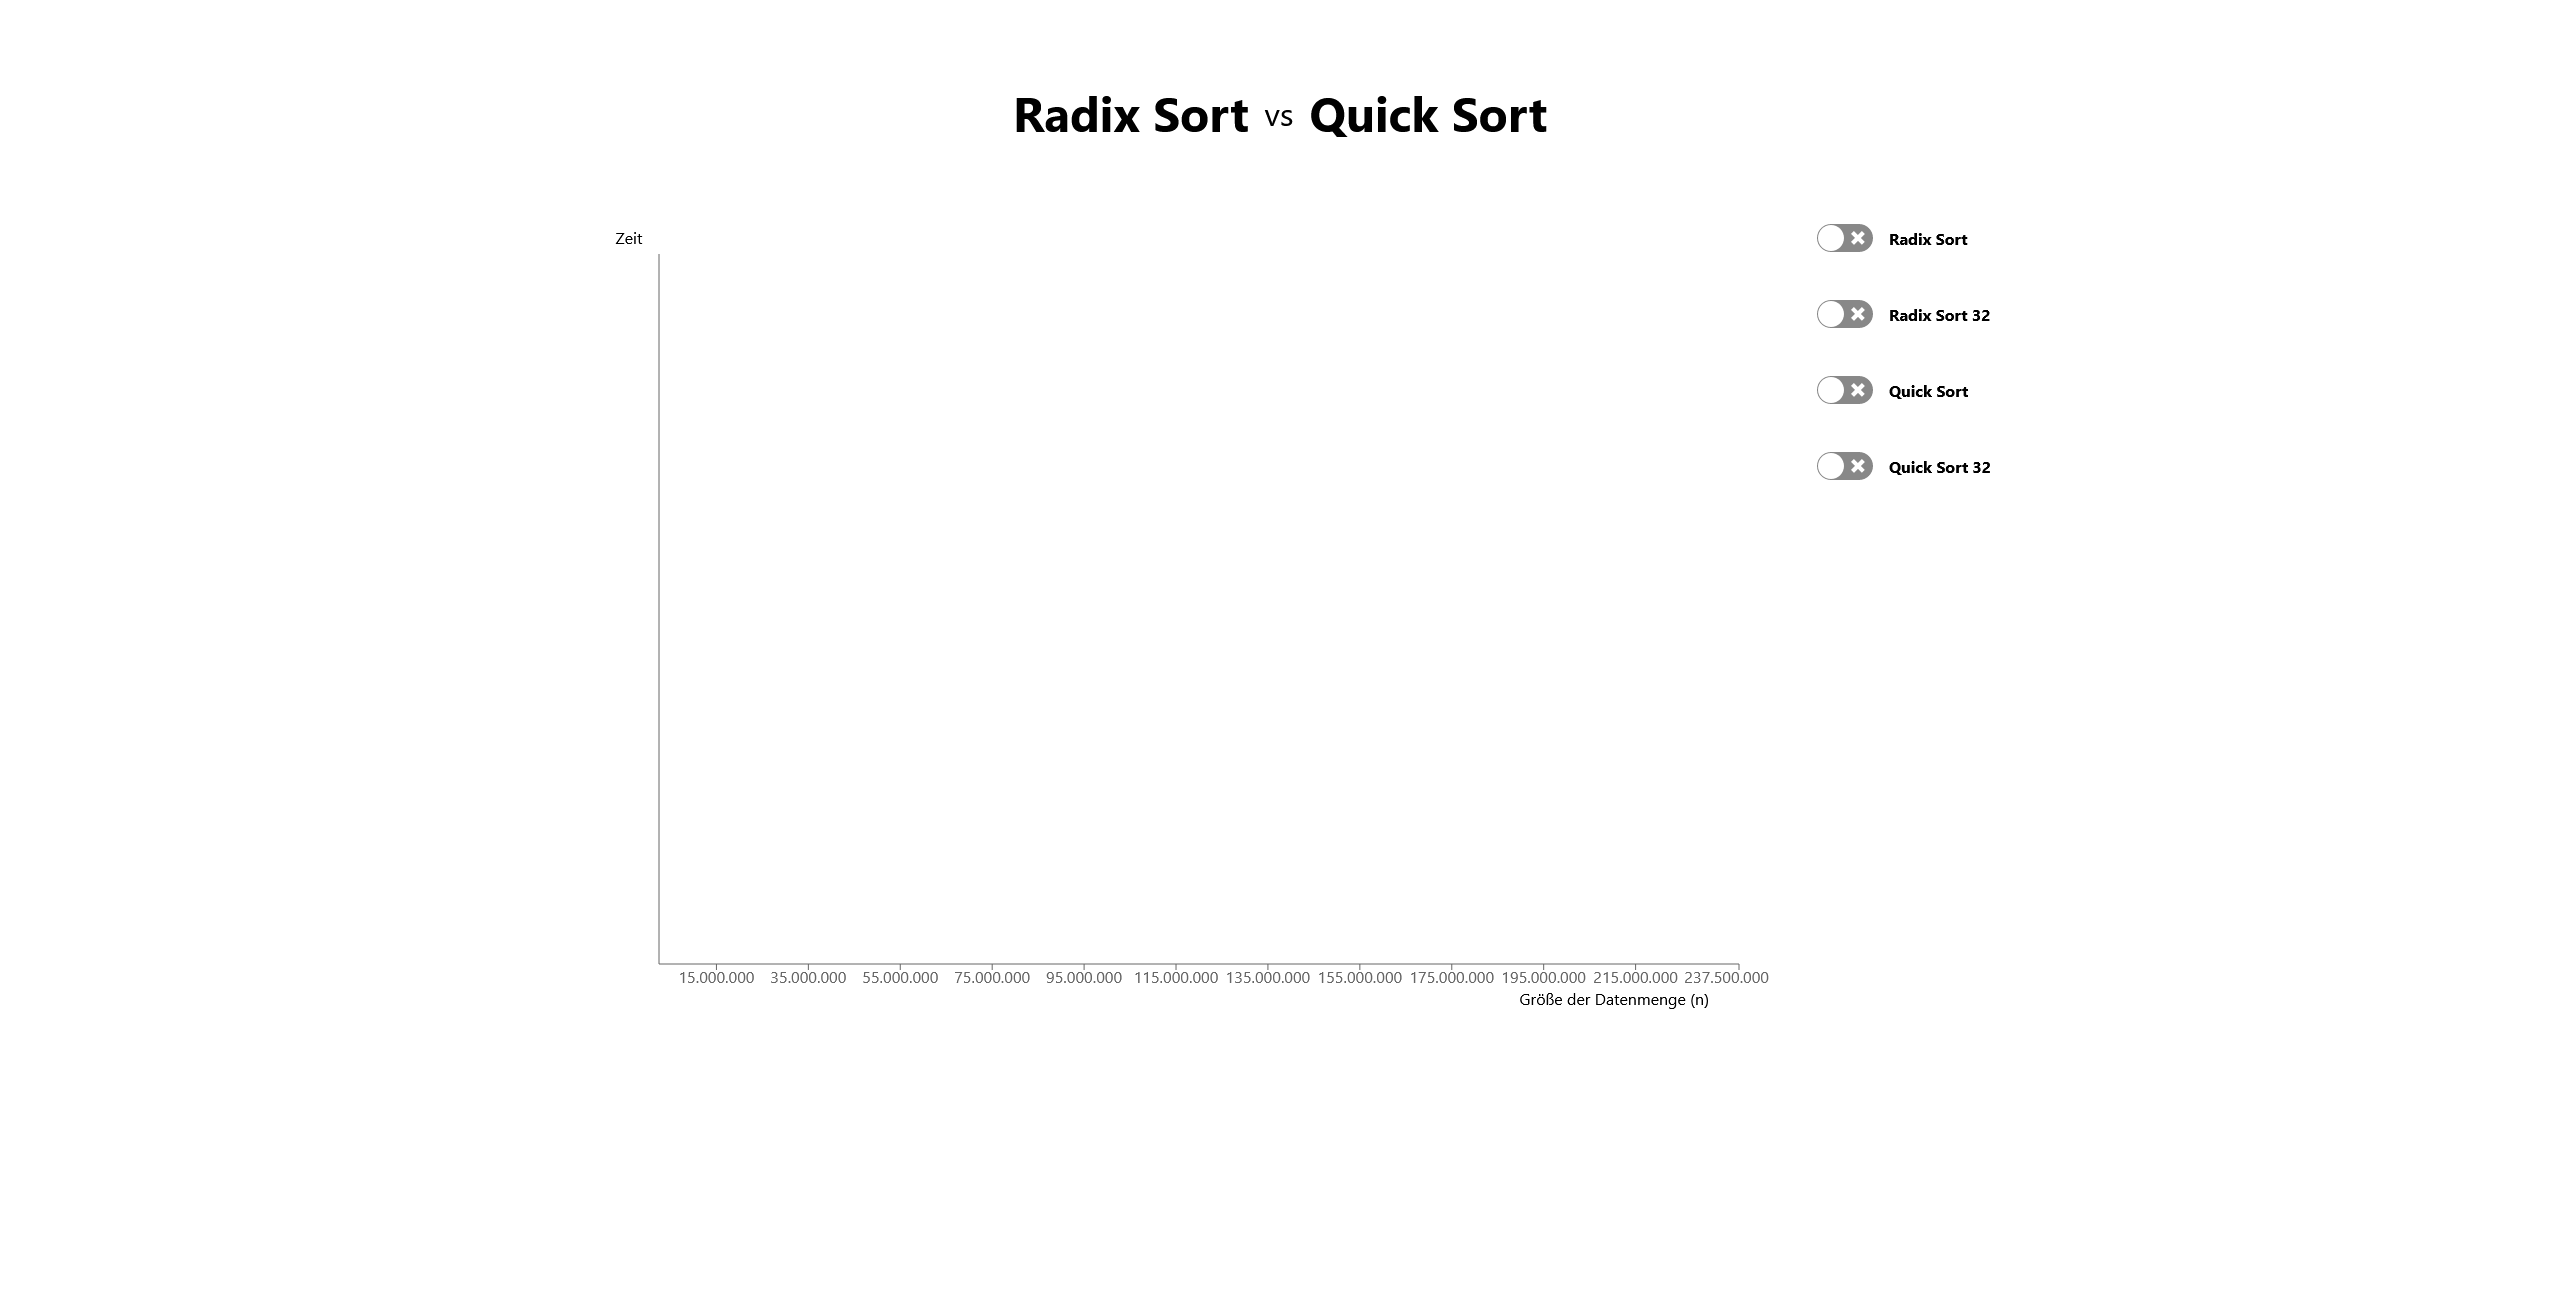
\includegraphics[width=\linewidth]{Abbildung-14}}
        \caption{Abbildung 14}
    \end{figure}

    \begin{figure}
        \centering
        \fbox{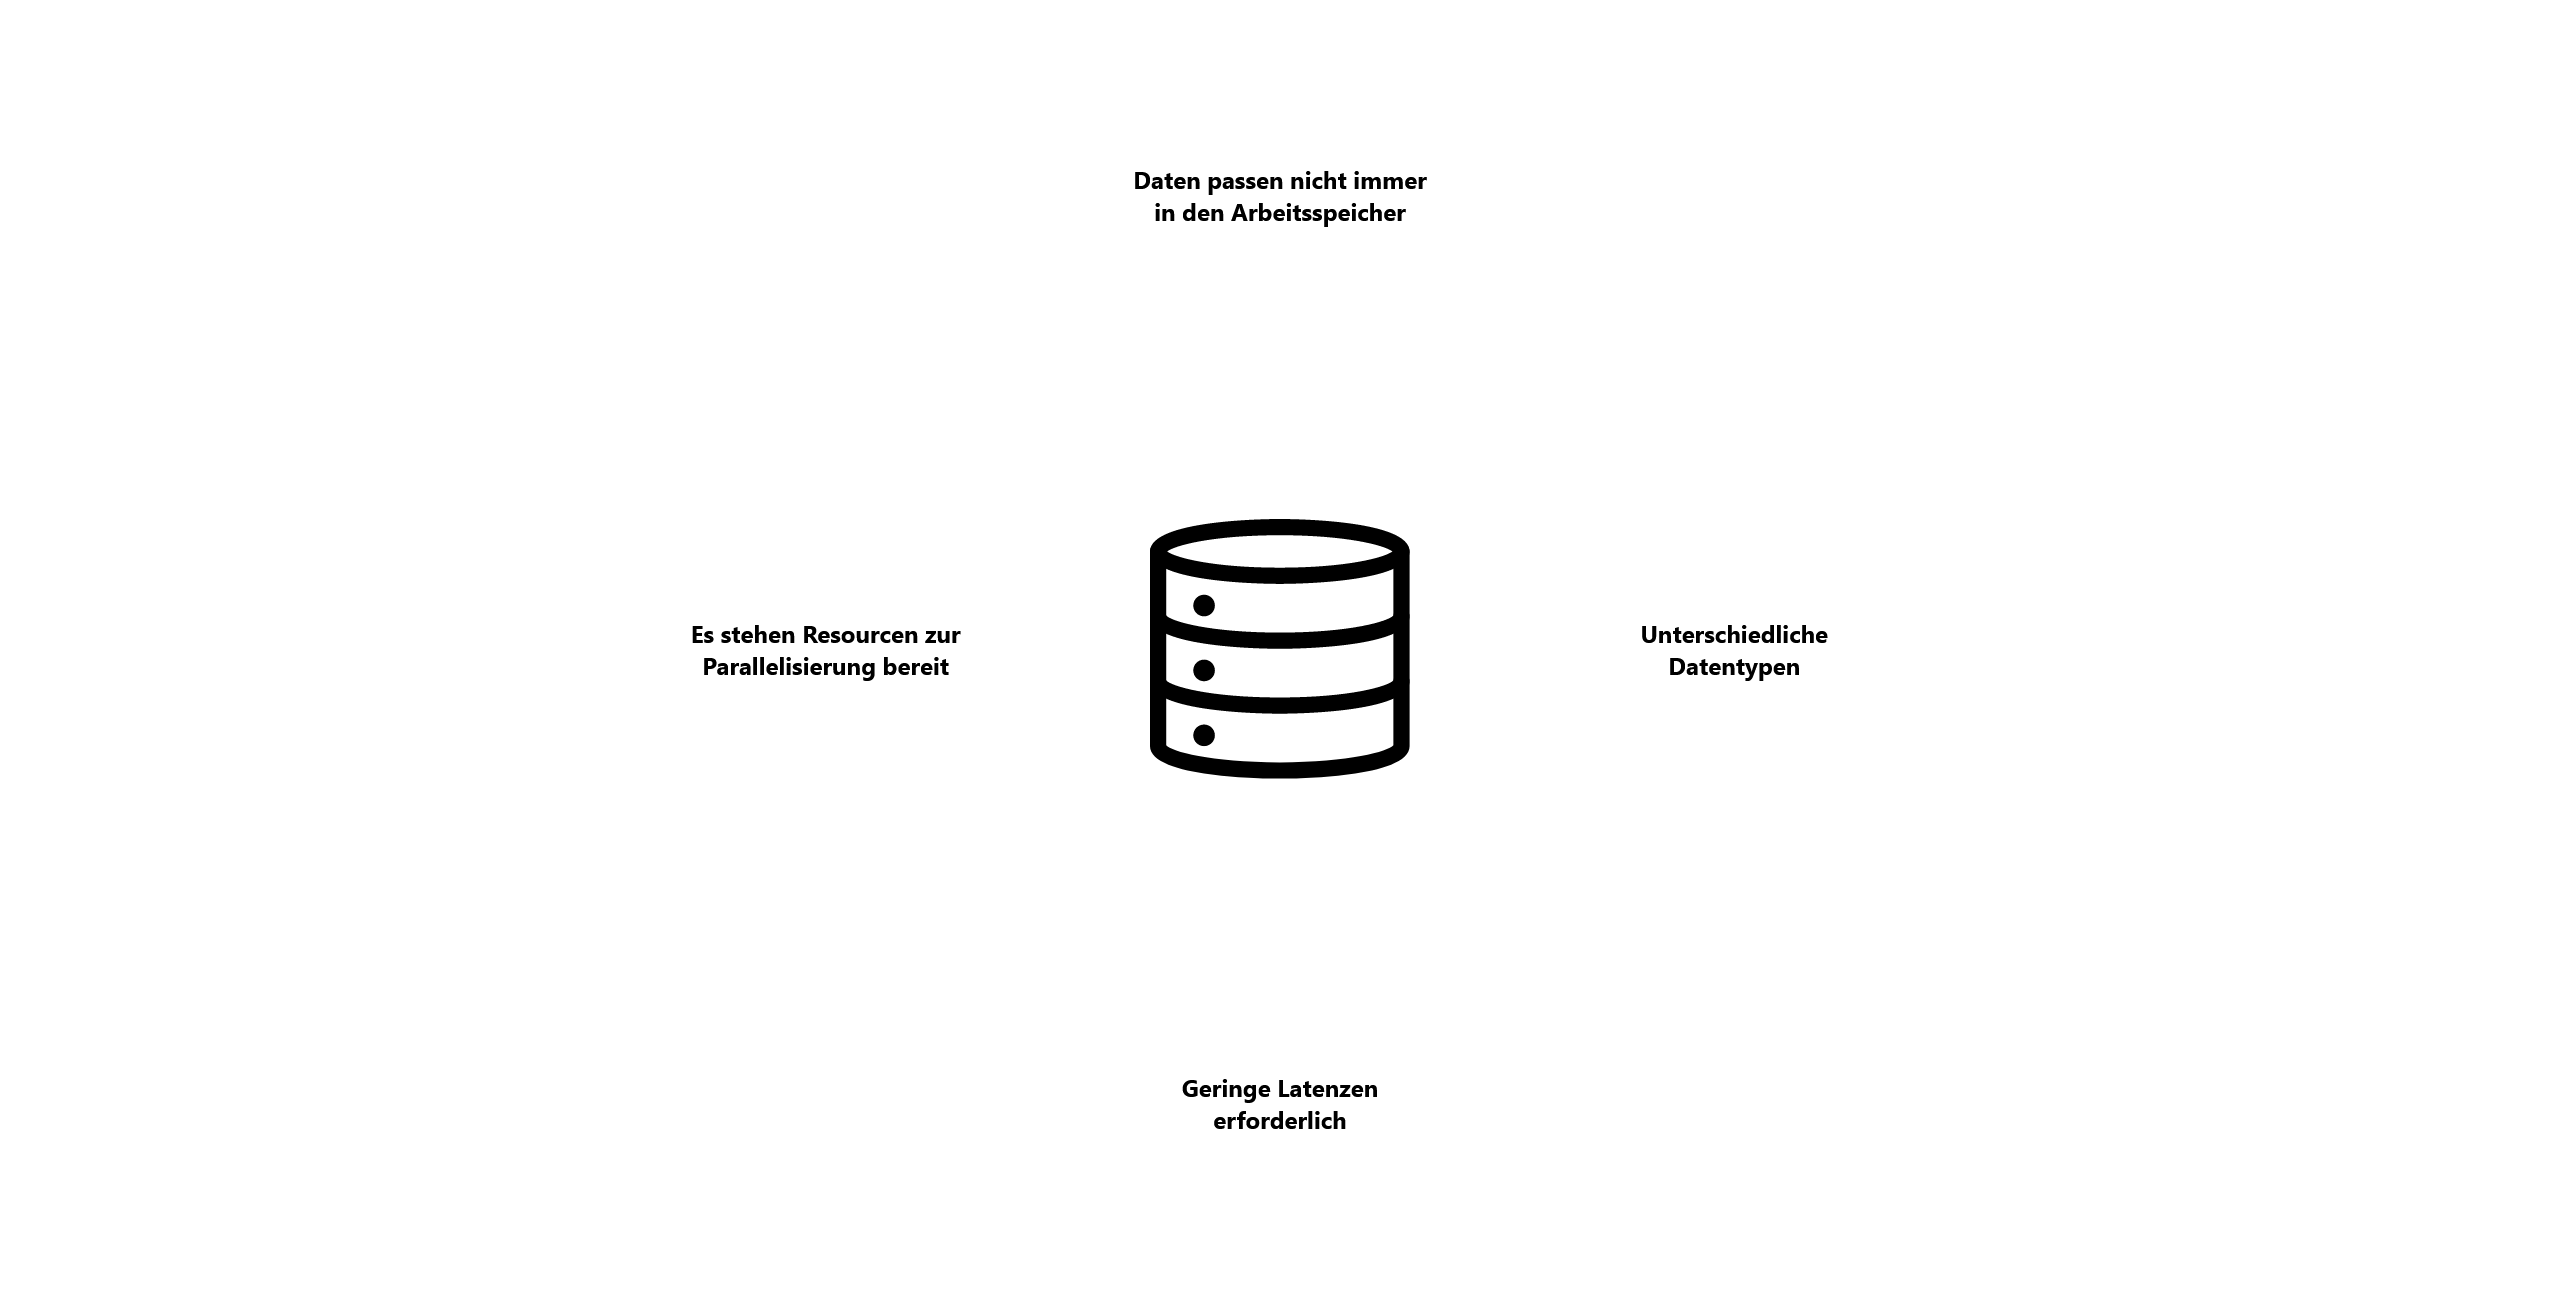
\includegraphics[width=\linewidth]{Abbildung-15}}
        \caption{Abbildung 15}
    \end{figure}

    \begin{figure}
        \centering
        \fbox{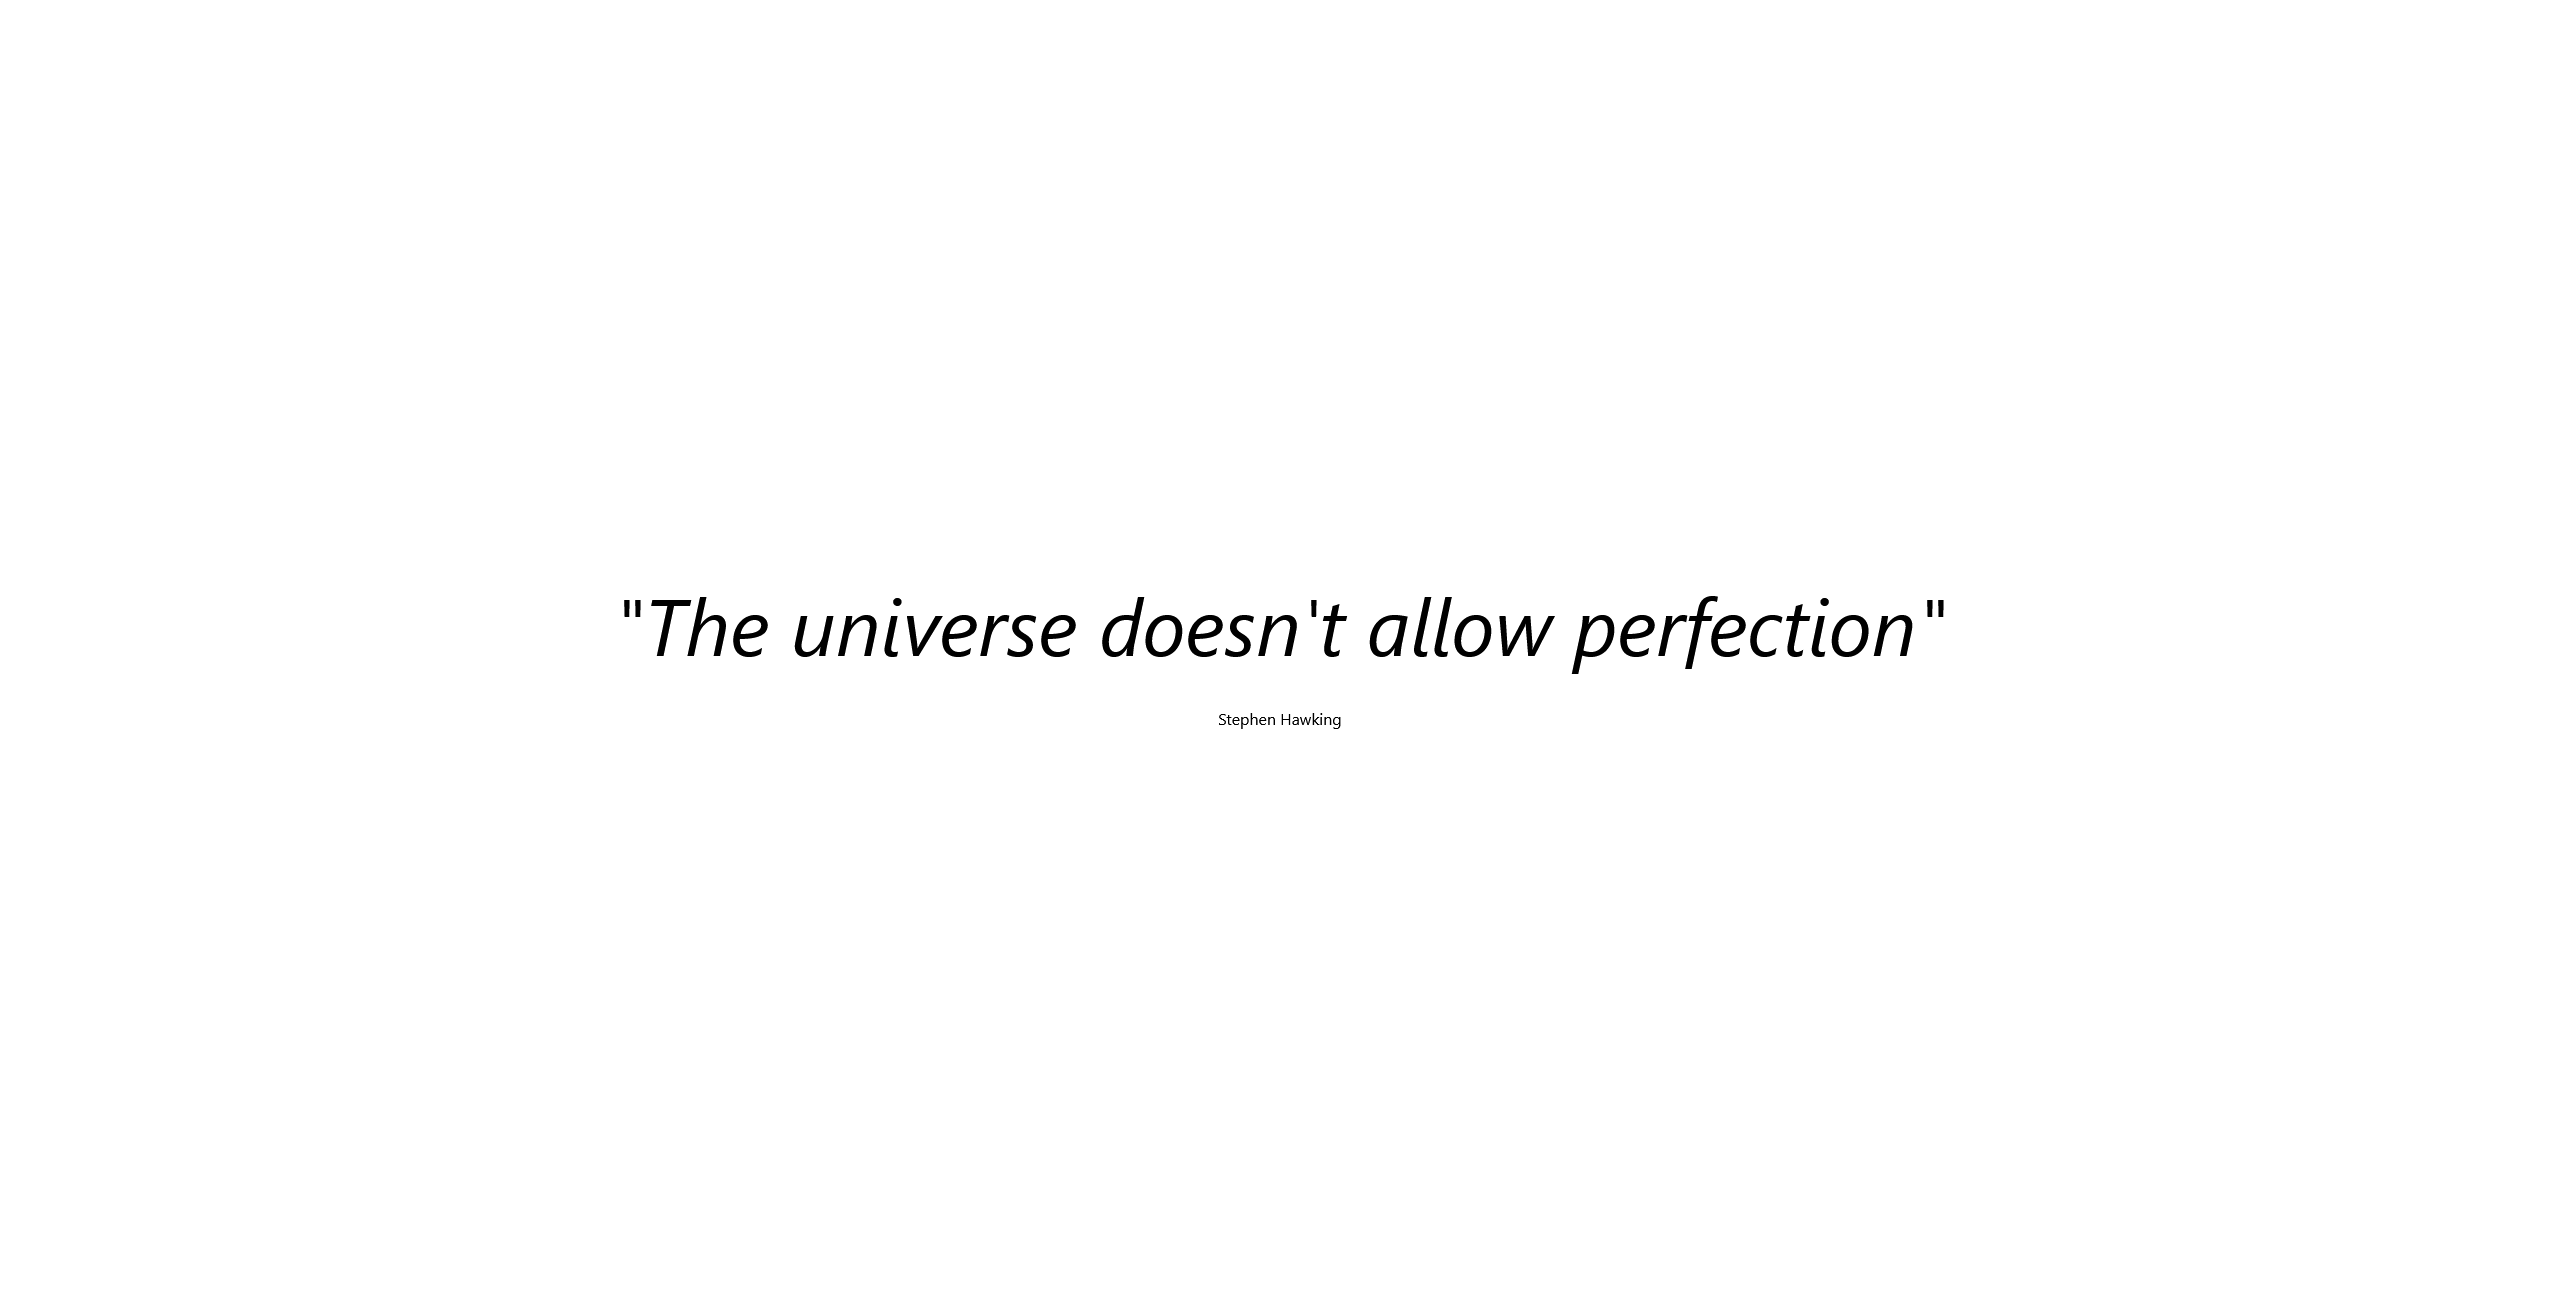
\includegraphics[width=\linewidth]{Abbildung-16}}
        \caption{Abbildung 16}
    \end{figure}

    \begin{figure}
        \centering
        \fbox{
\includegraphics[width=\linewidth]{Abbildung-17}}
        \caption{Abbildung 17}
    \end{figure}

    \begin{figure}
        \centering
        \fbox{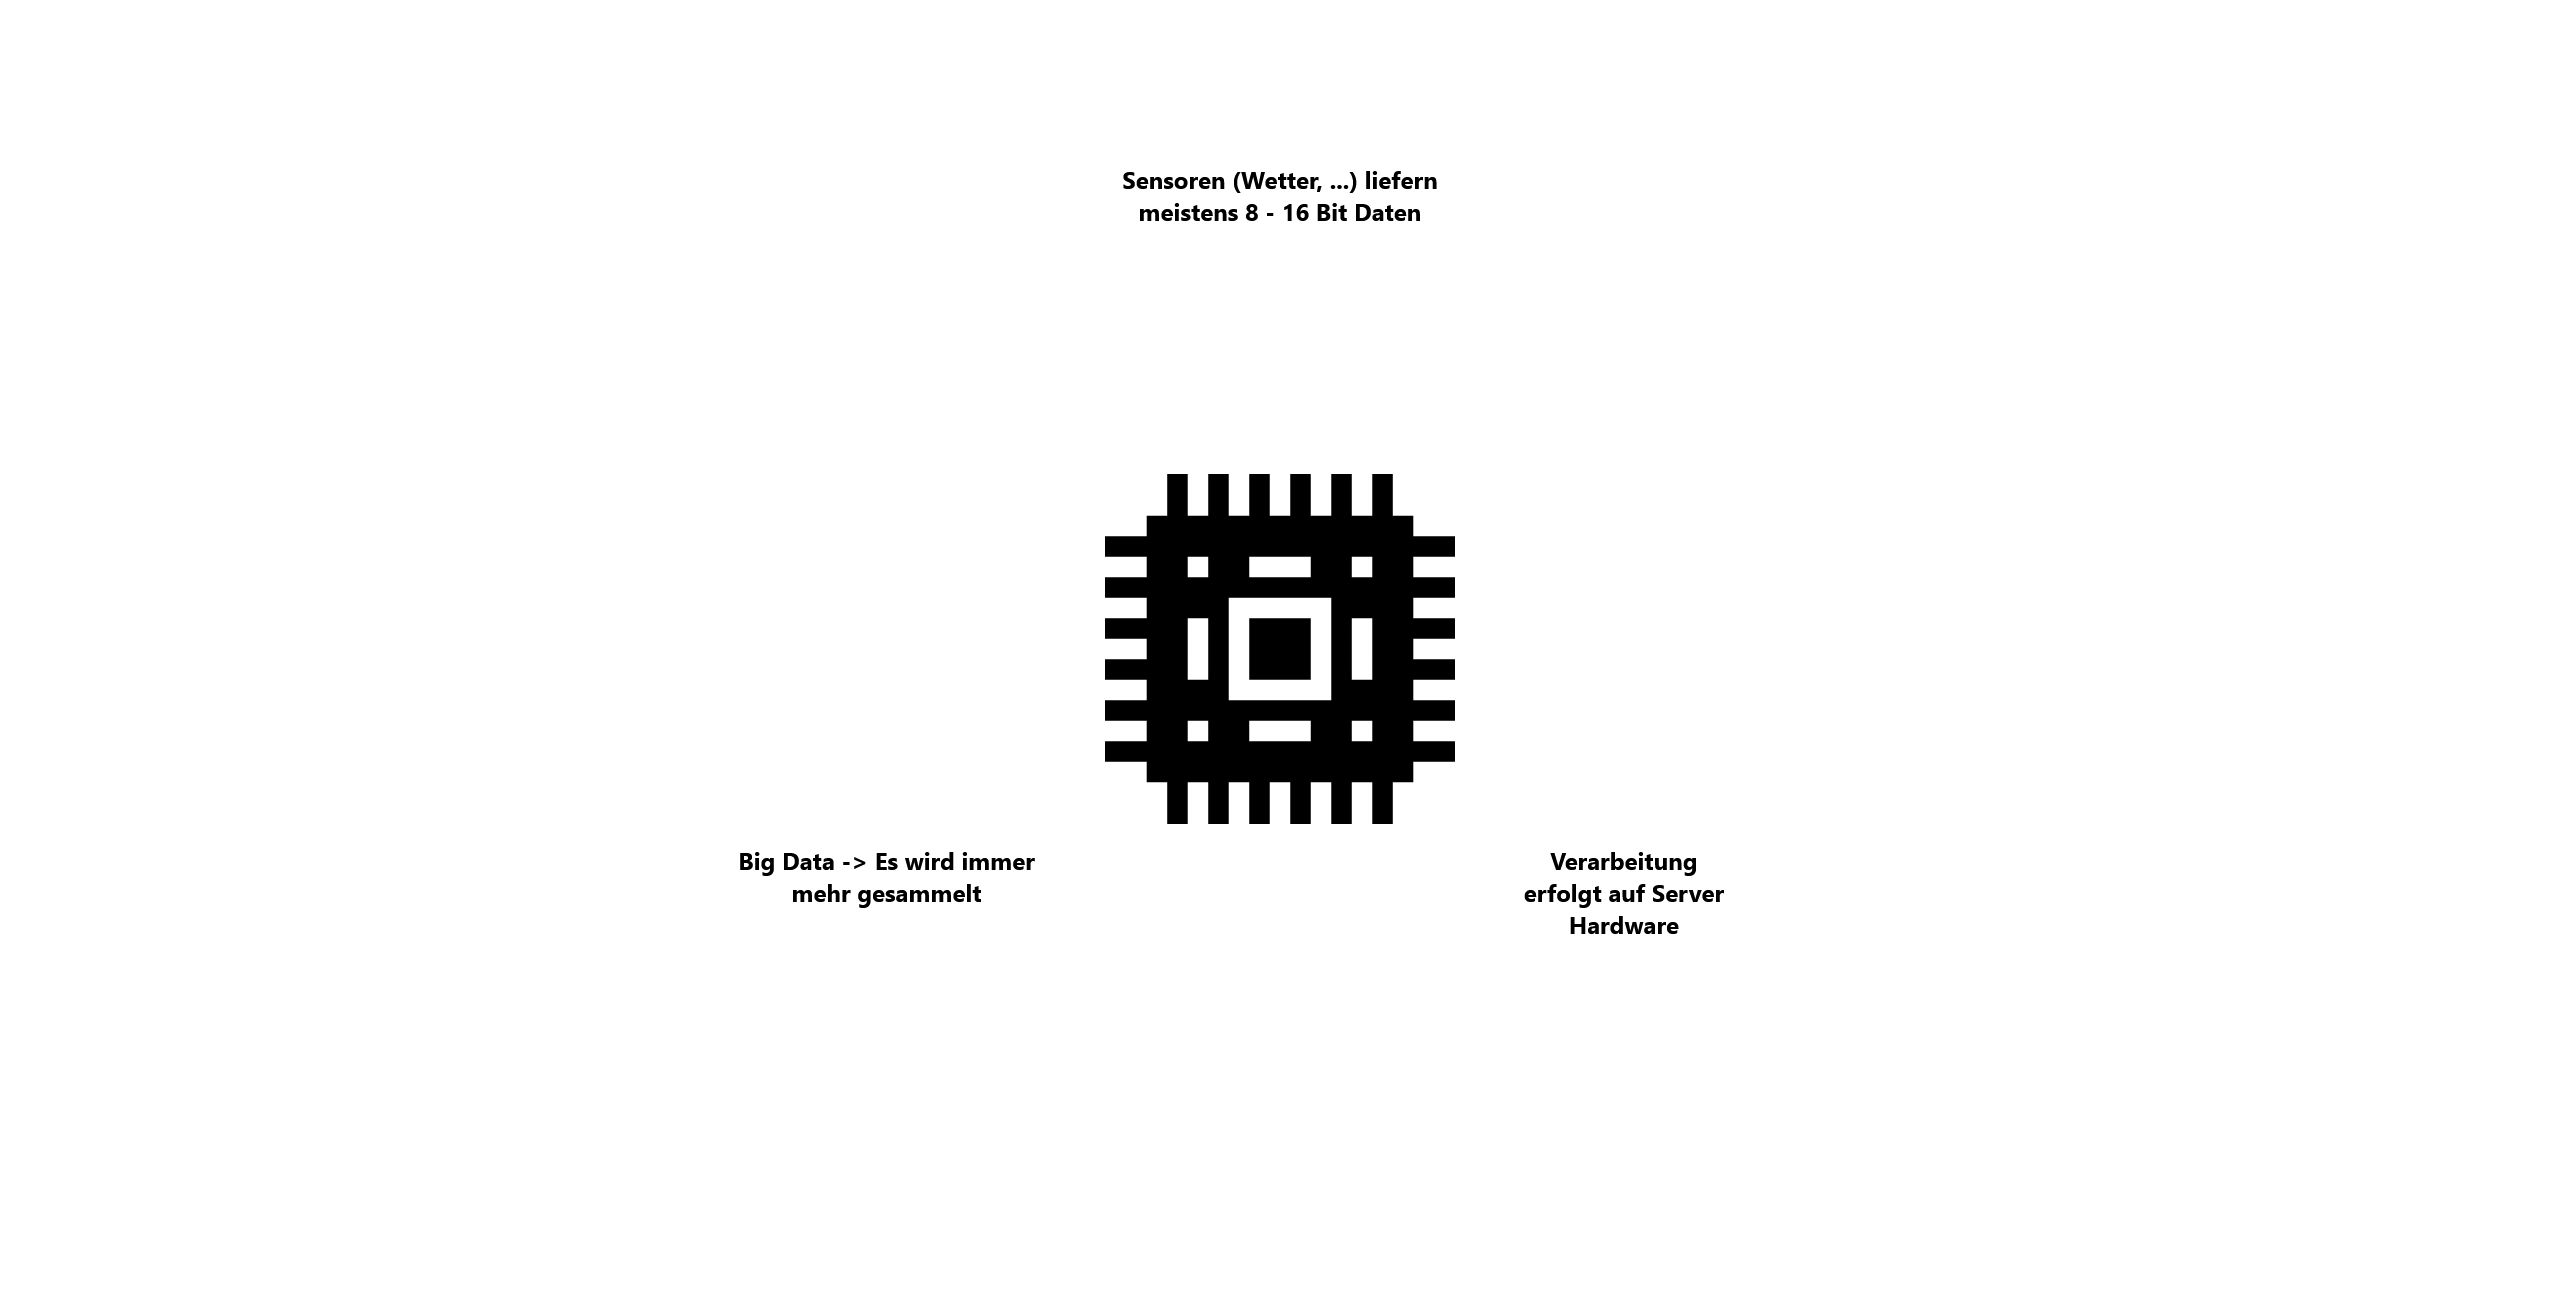
\includegraphics[width=\linewidth]{Abbildung-18}}
        \caption{Abbildung 18}
    \end{figure}

    \begin{figure}
        \centering
        \fbox{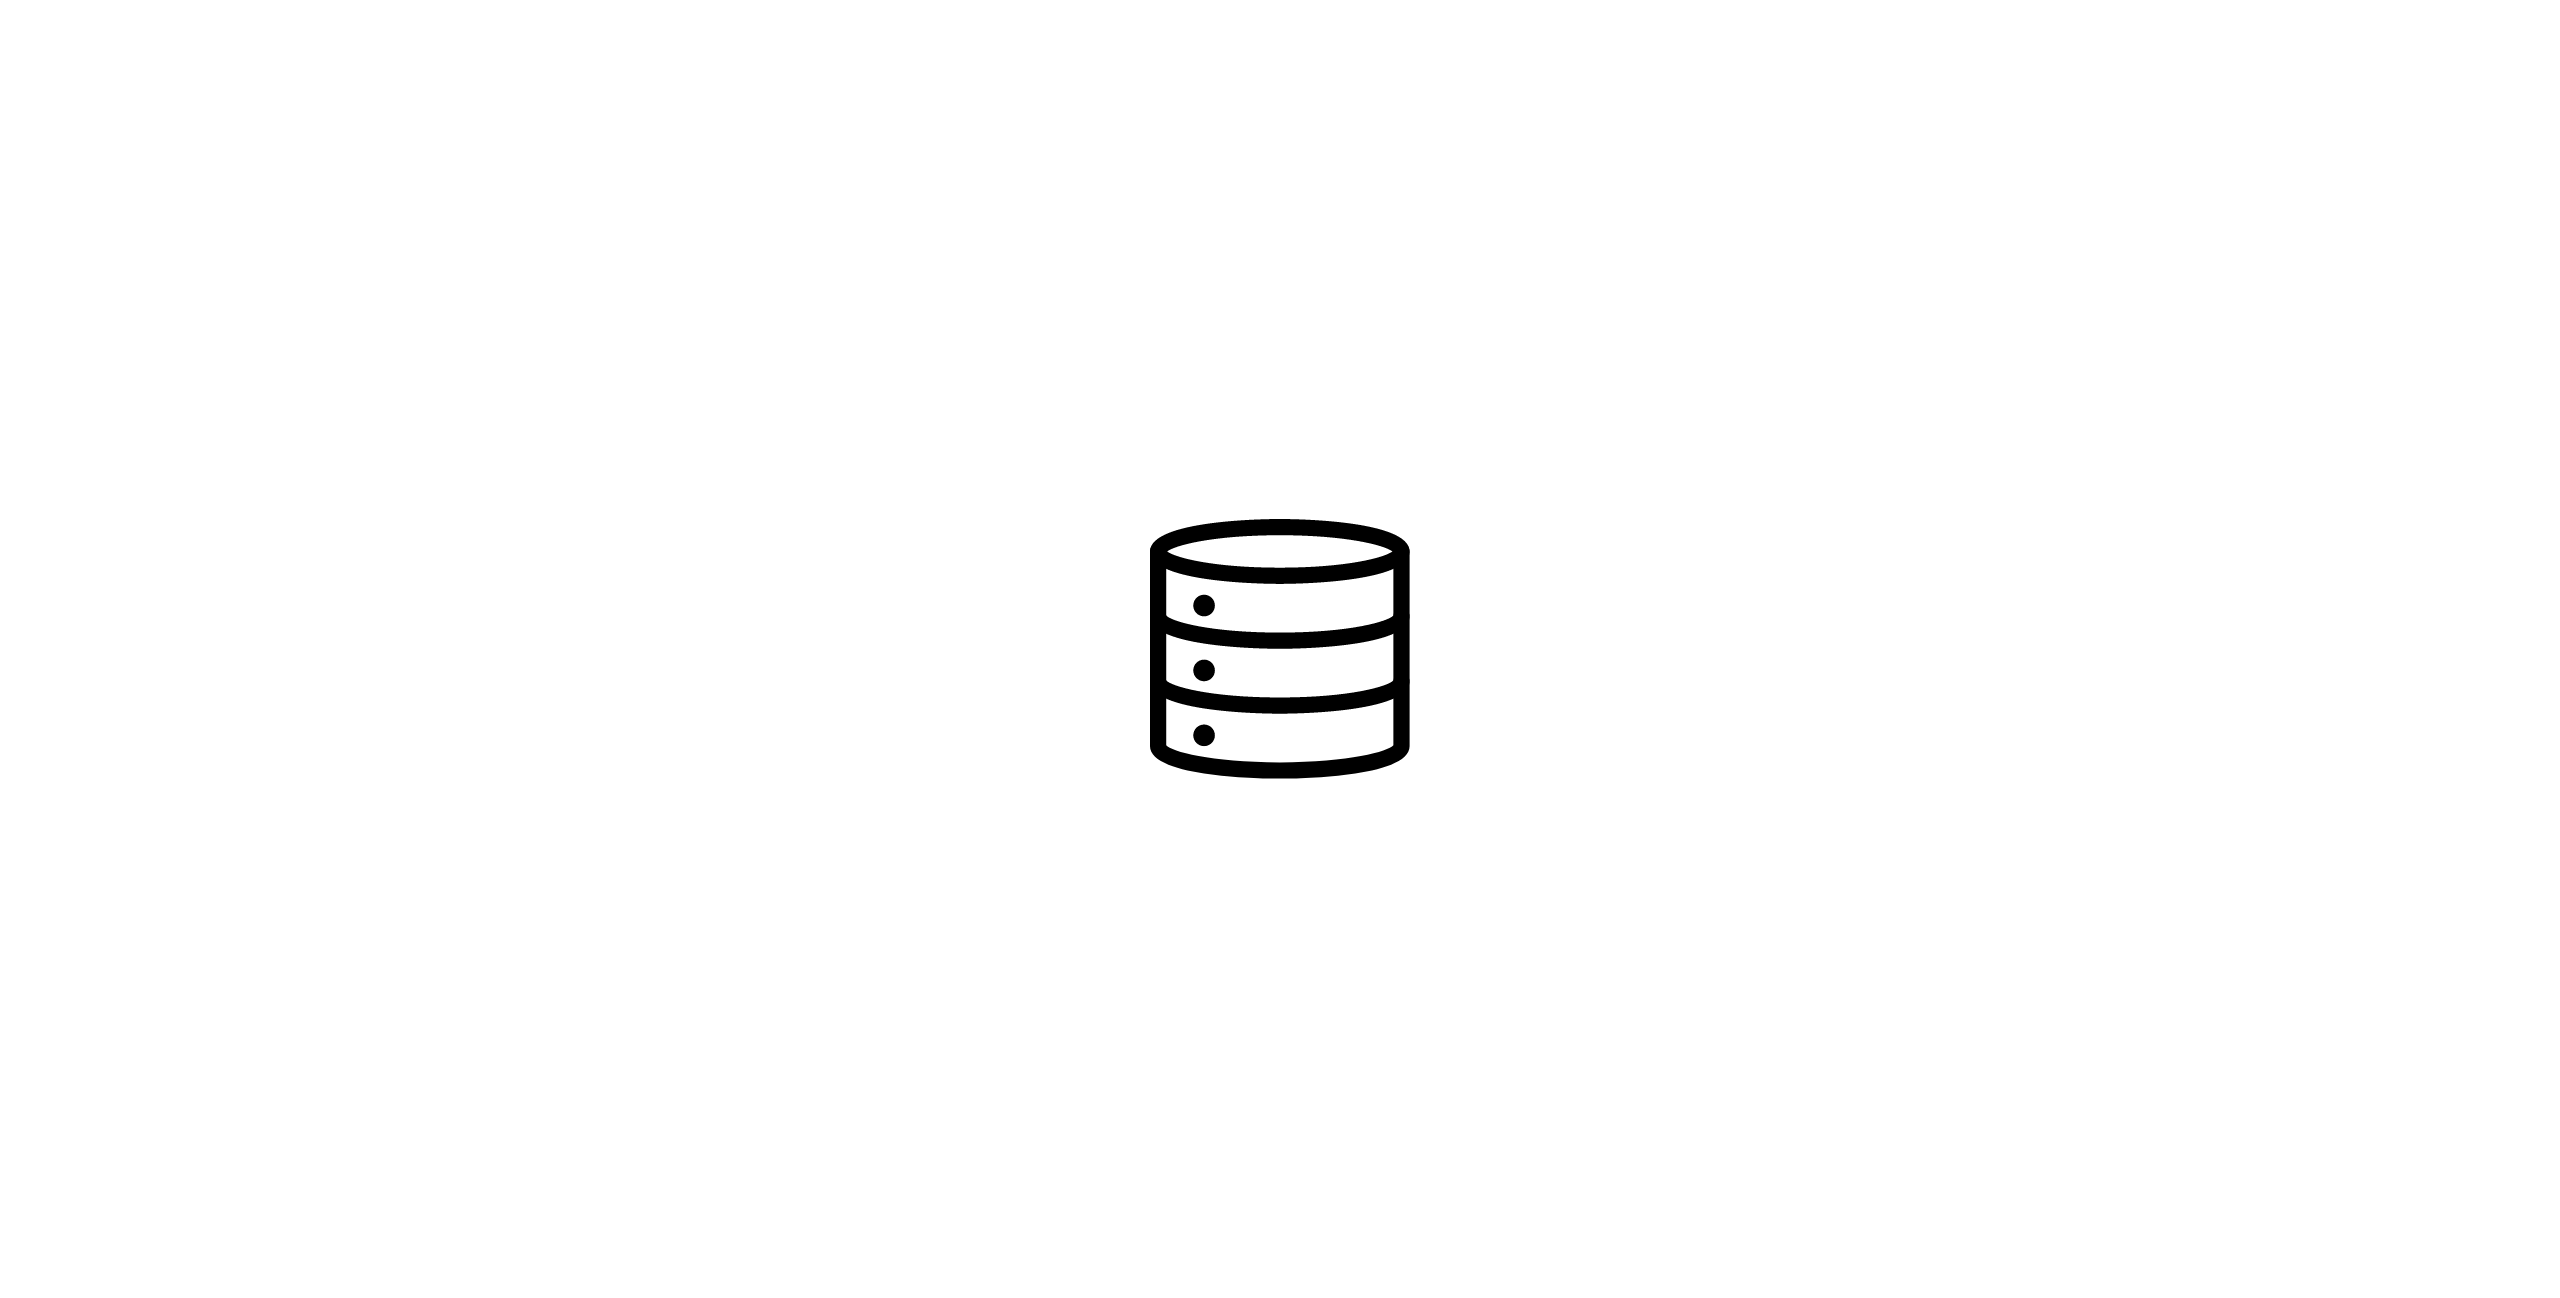
\includegraphics[width=\linewidth]{Abbildung-19}}
        \caption{Abbildung 19}
    \end{figure}

    \begin{figure}
        \centering
        \fbox{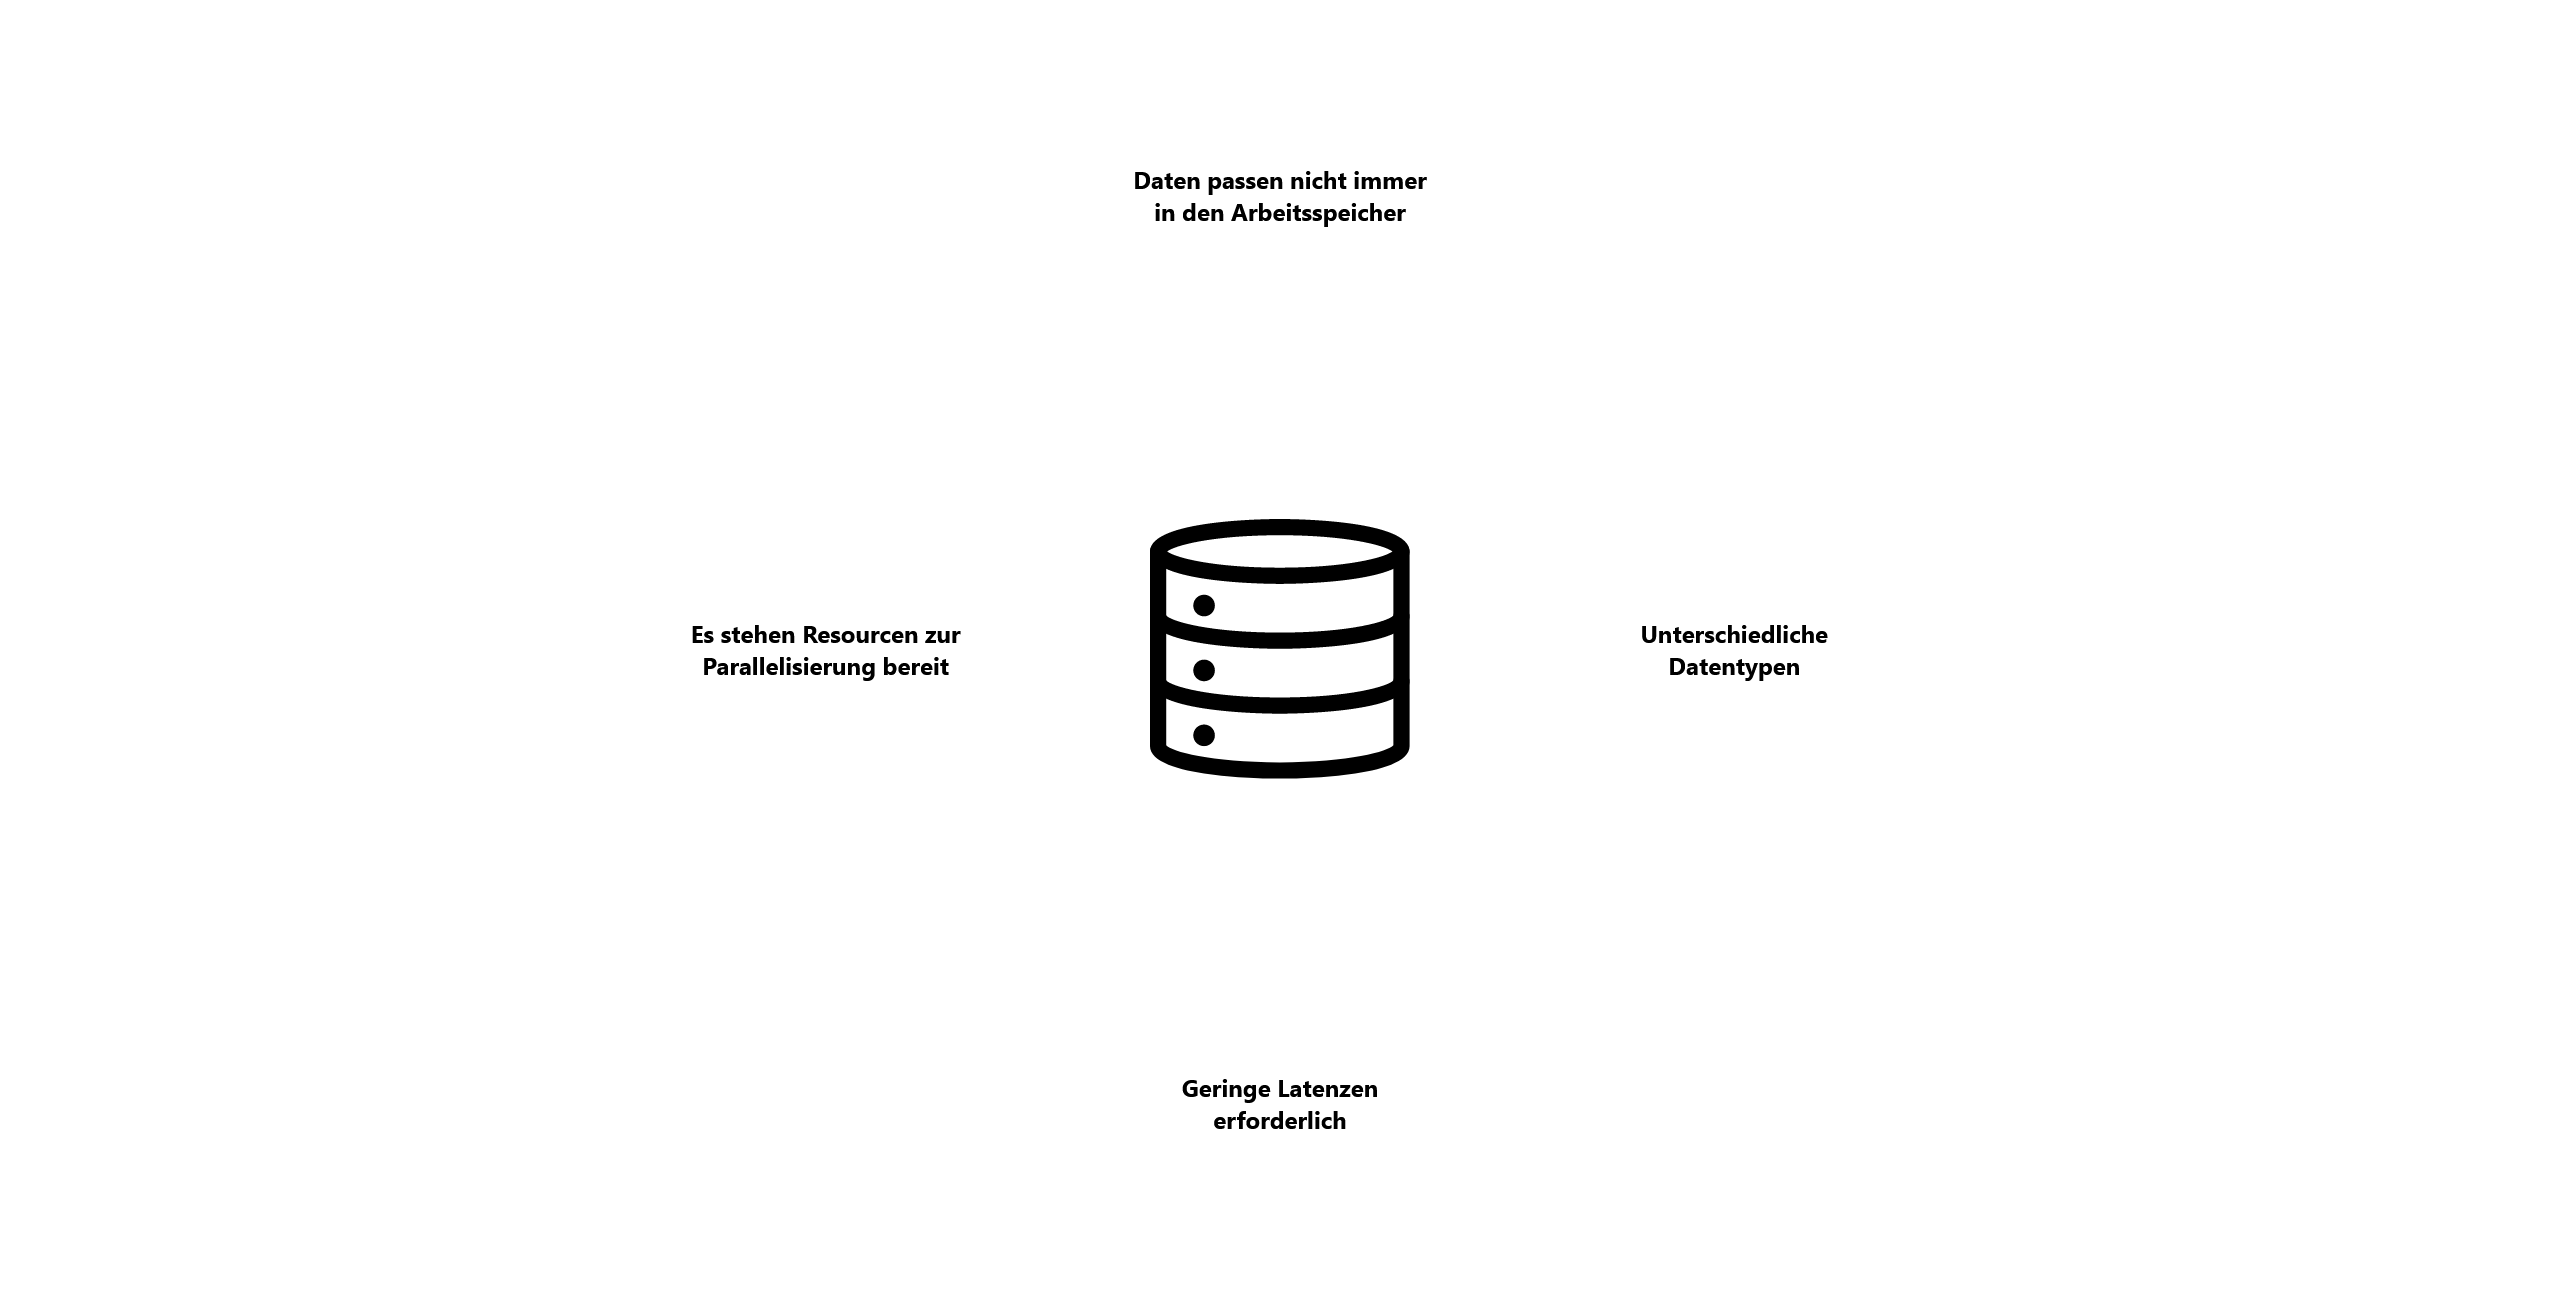
\includegraphics[width=\linewidth]{Abbildung-20}}
        \caption{Abbildung 20}
    \end{figure}

    \begin{figure}
        \centering
        \fbox{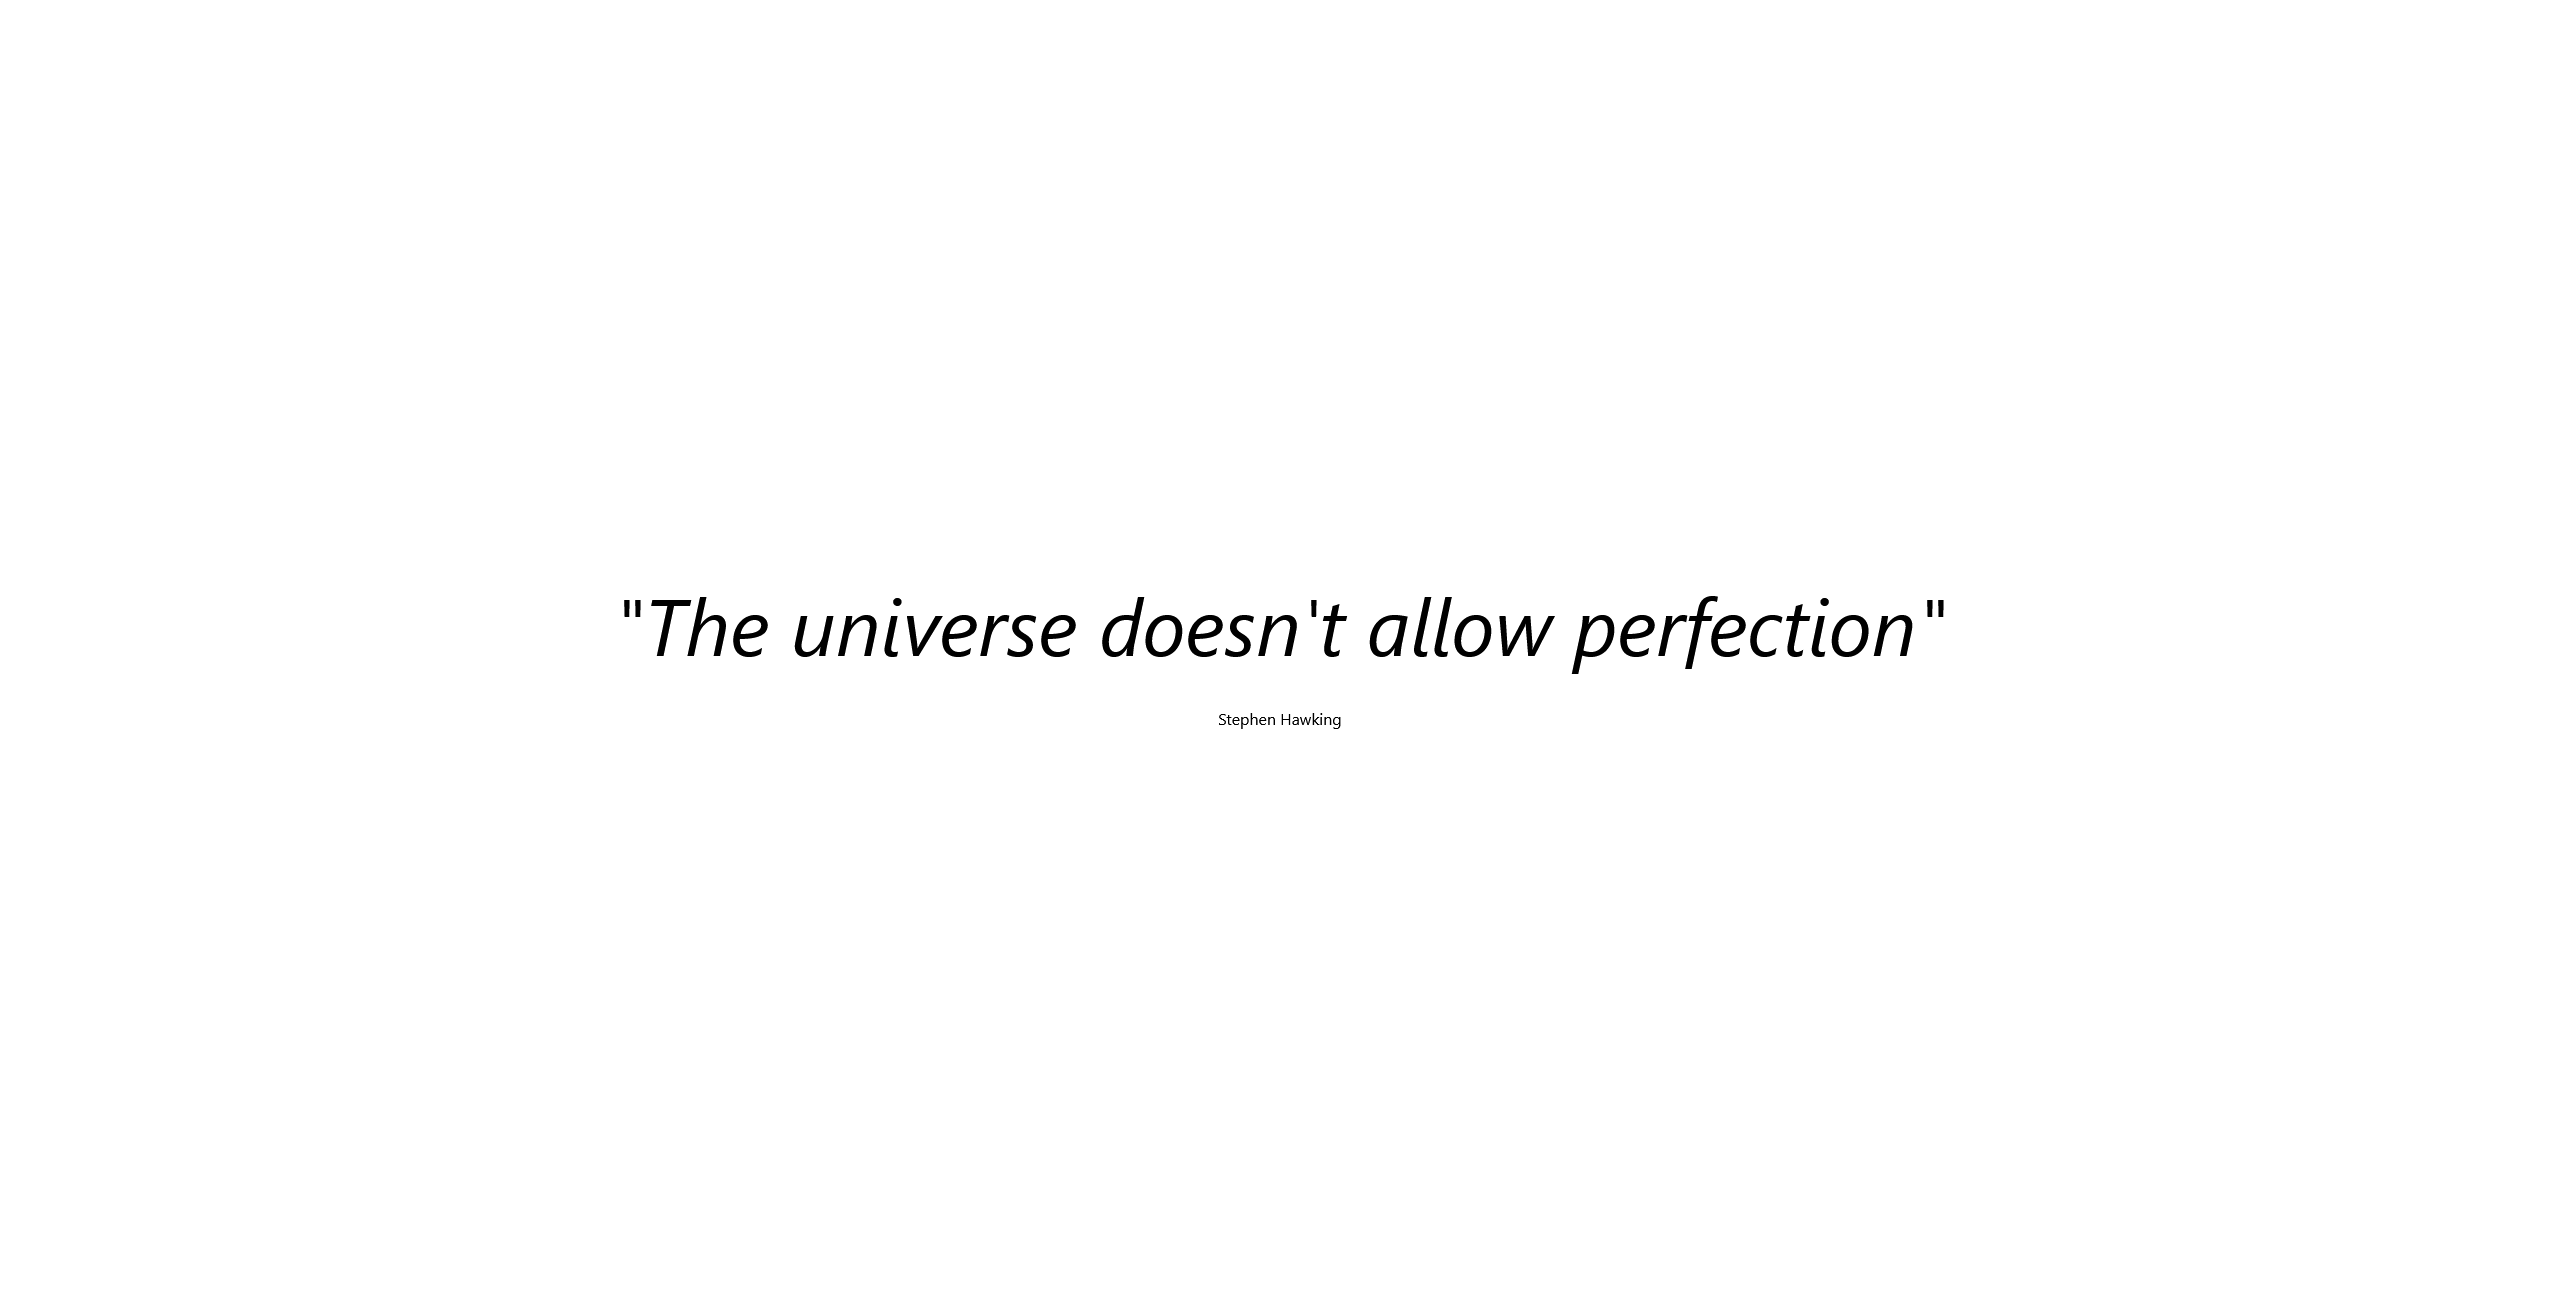
\includegraphics[width=\linewidth]{Abbildung-21}}
        \caption{Abbildung 21}
    \end{figure}

\end{document}
